\documentclass[12pt,halfparskip,DIV11,BCOR10mm]{scrreprt}

\usepackage{pystructure}

\usepackage{svn} % For handling of SVN keywords
\SVN $LastChangedDate$

\begin{document}

\begin{titlepage}

\pagenumbering{alph}
\thispagestyle{empty}

\begin{center}

\begin{figure}[h]
 \centering
 \vspace{0,5cm}
 
\includegraphics[width=\textwidth]{img/hsr_logo}
\end{figure}

\vspace{1cm}
{\Huge \bfseries PyStructure -- Automated Structure and Dependency Analysis of Python Code}

\vspace{0,5cm}
{\Large \bfseries Bachelor Thesis: Spring 2008}

\vspace{0,5cm}
\SVNDate{} (\textsc{Draft Version}) % TODO: delete

\vspace{0.5cm}
\begin{figure}[h]
 \centering
 
\includegraphics[width=5cm]{img/pystructure}
\end{figure}

\vspace{0.5cm}
Reto Schüttel \\ \url{reto@schuettel.ch}

\vspace{0,4cm}
Robin Stocker \\ \url{robin@nibor.org}

\vspace{0,4cm}
Supervised by Prof. Peter Sommerlad % TODO: e-mail address?

% FIXME external partner

\vspace{1cm}
\url{http://pystructure.ifs.hsr.ch/}

\end{center}
\end{titlepage}


\pagenumbering{roman}
\pagestyle{plain}

%%%%%%%%%%%%%%%%%%%%%%%%%%%%%%%%%%%%%%%%%%%%%%%%%%%%%%%%%%%%%%%%%%%%%%%
\chapter*{Abstract}

A vital part of software development is defining a good architecture when planning a project. But during implementation, the intended structures are often neglected and the program's architecture grows in a different way than planned – a problem called \emph{architectural decay}. When only looking at source code, tracking the architecture and keeping a high-level view of dependencies between components is difficult. Commonly used graphical models such as domain or architecture diagrams are helpful, but they usually just describe the \emph{intended} design, rather than the \emph{actual} structure.

PyStructure's goal was to develop an analyser which reveals these internal structures and dependencies in a Python program by statically analysing its source code. Dependencies are identified by determining what types are used in a particular component. But as Python is a dynamically typed language, types are not known before the application is run. Therefore a major aspect of the project was to develop an algorithm, called type inferencer, which deduces types by mimicking the evaluation process of the Python interpreter.

The following details are extracted by the structural analyser:

\begin{itemize}
    \item All involved components such as modules, classes and methods
    \item Dependencies between these components caused by:
    \begin{itemize}
        \item Method calls
        \item Variables, arguments or attributes of a certain type
        \item Inheritance
    \end{itemize}
\end{itemize}

The extracted data can be visualised by Structure 101g, a program developed by Headway Software. Structure 101g shows dependencies as graphs in various levels of detail and provides a wide variety of analysis tools, like detecting cyclic dependencies or validating the current architecture. This allows to effectively monitor the progress of a project's architecture during development.

The structural data itself is also useful in other areas of software development like enhanced accuracy for automatic refactoring or better support for code completion in integrated development environments.

%PyStructure is available under the open source license LGPL from http://pystruture.ifs.hsr.ch/.


%%%%%%%%%%%%%%%%%%%%%%%%%%%%%%%%%%%%%%%%%%%%%%%%%%%%%%%%%%%%%%%%%%%%%%%
\chapter*{Management Summary}

\section*{Motivation}

Keeping software manageable and simple as it grows is a very challenging tasks. 
It is not only important to define a good architecture when planning a project, but also to continuously compare it to the actual implementation. Tracking the architecture and keeping a high-level view of dependencies between components is difficult when only looking at source code. Graphical models such as domain or architecture diagrams help, but the problem with them is that they are disconnected from the source code and might not be completely accurate.

Manually checking a program's structure is time consuming and error prone and is therefore not very practical. A more preferable solution would be to have an automatic way to visualise the structure of a project. This would also be generally useful when exploring the innards of an unfamiliar code base or while evaluating the impact of a particular change.

\section*{Goal}

PyStructure's goal was to develop an analyser which reveals these internal structures and dependencies in a Python program by statically analysing its source code. Dependencies are identified by determining what types are used in a particular component. But as Python is a dynamically typed language, types are not known before the application is run. Therefore a major aspect of the project was to develop an algorithm, called type inferencer, which deduces types by mimicking the evaluation process of the Python interpreter.

As part of a previous project about refactoring support for Python called PEPTIC \cite{peptic2}, we developed a basic version of such a type inferencer. For PyStructure it was decided to reuse this type inferencer and develop it further to make it usable as a base for structure analysis.

PyStructure should be able to export the structure and dependency data to Structure 101g, a structure visualisation program developed by Headway Software. It shows dependencies as graphs in various levels of detail and provides a wide variety of analysis tools, like detecting cyclic dependencies or validating the current architecture.

\section*{Results}

In the 16 weeks of the project we were able to accomplish most of the planned goals. PEPTIC's type inferencer was extracted and moved to an independent new project. It now supports almost all of Python's language features and is able to produce a sensible result in most cases.

The implemented structural analyser is able to extract a program's internal structure, consisting of packages, modules and classes, and to identify and evaluate all expressions that cause dependencies.

\section*{Outlook}

There is still room for improvements and optimisations for the type inference system, like:

\begin{itemize}
    \item The performance of the goal engine for bigger projects and in general can be improved very much. By doing better and more caching of goals, similar calculations can be done only once without sacrificing the precision of the results.
    \item Support for more language constructs and built-in types can be added.
    % rschuett: Was noch?
\end{itemize}

The PEPTIC project still uses the old type inference engine for refactorings, because the new engine has been developed in a separate repository. For the refactorings to make use of the new features, the code has to be ported to the new engine. This will probably also lead to changes to the type inference system itself, because we did not take special care for the requirements of an IDE during this project.

\newpage

\tableofcontents

\newpage
\pagenumbering{arabic}
\pagestyle{scrheadings}

%%%%%%%%%%%%%%%%%%%%%%%%%%%%%%%%%%%%%%%%%%%%%%%%%%%%%%%%%%%%%%%%%%%%%%%
\chapter{Introduction}

\section{Structural Analysis}

There are a number of areas where structural analysis is useful:

\begin{wrapfigure}{r}{6cm}
    \vspace{-0.3cm}
    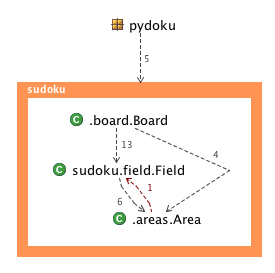
\includegraphics[width=6cm, trim=10 10 10 10, clip=true]{dependencies}
    \vspace{-1cm}
\end{wrapfigure}

\paragraph{Architecture}
Keeping software manageable and simple as it grows is a very challenging tasks. Having a good idea from the beginning how the architecture of a software project should look like is very important. Equally important, but much more challenging is actually keeping the software within the planned architecture. It's quite easy to draw some boxes representing the different components on to a white board. But even for an experienced developer, it is hard to know all the time what should belong where and what is being used by it.

\paragraph{Isolating Components}
Or imagine that you need to extract a rather big part of an application into an independent piece of software. Without having a clear idea about a project's structure all one can do is to just remove the essential part and check the errors while running the program or during the compilation. Wouldn't it be nice if you could just select a part of your application, be it a method, a class or a whole package and an instant later you could see what a) is used by this particular component (dependencies) and b) what uses it (consumers).

\paragraph{Cycles}
Another common unpleasant situation is when two high level components have an interdependency. For example it is usual that a GUI has full access to the business logic, but if there's some part in the business logic which accesses the GUI the two components are mutual dependent on each other. Between high level components this is often undesired as this means that one component cannot work without the other.

% rstocker { 
This problems gets obvious for example when new requirement arises which asks for the business logic to be accessed as a web application. Suddenly bigger parts of both GUI and business logic would have to be refactored to accommodate the two different needs.
% } so okay?

It has to be said that mutual dependencies on the class level, just between classes, are completely normal and often inevitable.

\section{Type Inference}

Before any meaningful structure analysis of a program is possible???, the individual components have to be identified and analysed. To know what dependencies a component (e.g. a class) has, it first has to be determined what kind of other components are being used. For example if the GUI class calls a method of a class in the business logic we clearly have a dependency between these two components. It becomes obvious that knowing the type of a given expression, in this example the method call, is imperative for any meaningful structural analysis.

This leads to the question, how can the type of a given expression be determined? In Java the answer would be very simple to find, as an explicitly and statically typed language the type is always stated in the definition.\footnote{In the example \java{boolean isOdd(int i)}, method \java{isOdd} has a parameter \java{i} with the type \type{int} and returns a \type{boolean}.} Python, on the other hand, is a \emph{dynamically} typed language. Types aren't specified at all, they are only known at runtime by the interpreter. To still be able to determine them, a heuristic has to be used which infers the types by looking at the context and finding answers to questions like ``Where was the variable defined?'' and ``Who called that function?''. This heuristic is usually called type inferencer (TI). As the term \emph{heuristic} implies is it impossible to evaluate the type in every case, in certain cases assumptions have to be made.

\subsection{Goal}

So, developing a type inferencer was a central goal of the project. To be useful for structural analysis, it should be able to resolve the type of the following components:

\begin{itemize}
    \item Local \& global variables
    \item Arguments
    \item Attributes
    \item Return values of functions \& methods
\end{itemize}

Of course the type inferencer should take the application as a whole into account and develop a best guess what the given expression's type could be. For example, in the case of a method argument, the type inferencer should look for all places where the particular method is called and what argument type was used.

The type inferencer should also be able to handle the case where more than one type is possible for a single expression, a simple example\footnote{The ternary operator is a bit different in Python than in other languages, the example means: \java{vehicle = (input == "car") ? Car() : Plane()}} would be:

\begin{lstlisting}
vehicle = Car() if input == "car" else Plane()
\end{lstlisting}

In this case the type inferencer has to detect that \code{vehicle} can be of type \type{Car} or \type{Plane}.

\subsection{Process Overview}

The type inferencer is divided into three main process stages:

\begin{itemize}
    \item \textbf{Parser} – Parses source code and generates an abstract syntax tree (AST)
    \item \textbf{Definition Visitor} – Builds a model of the program (modules, classes, methods, related variables)
    \item \textbf{Type Inferencer} – Evaluates the type of an expression
\end{itemize}

\begin{figure}[h!]
 \centering
 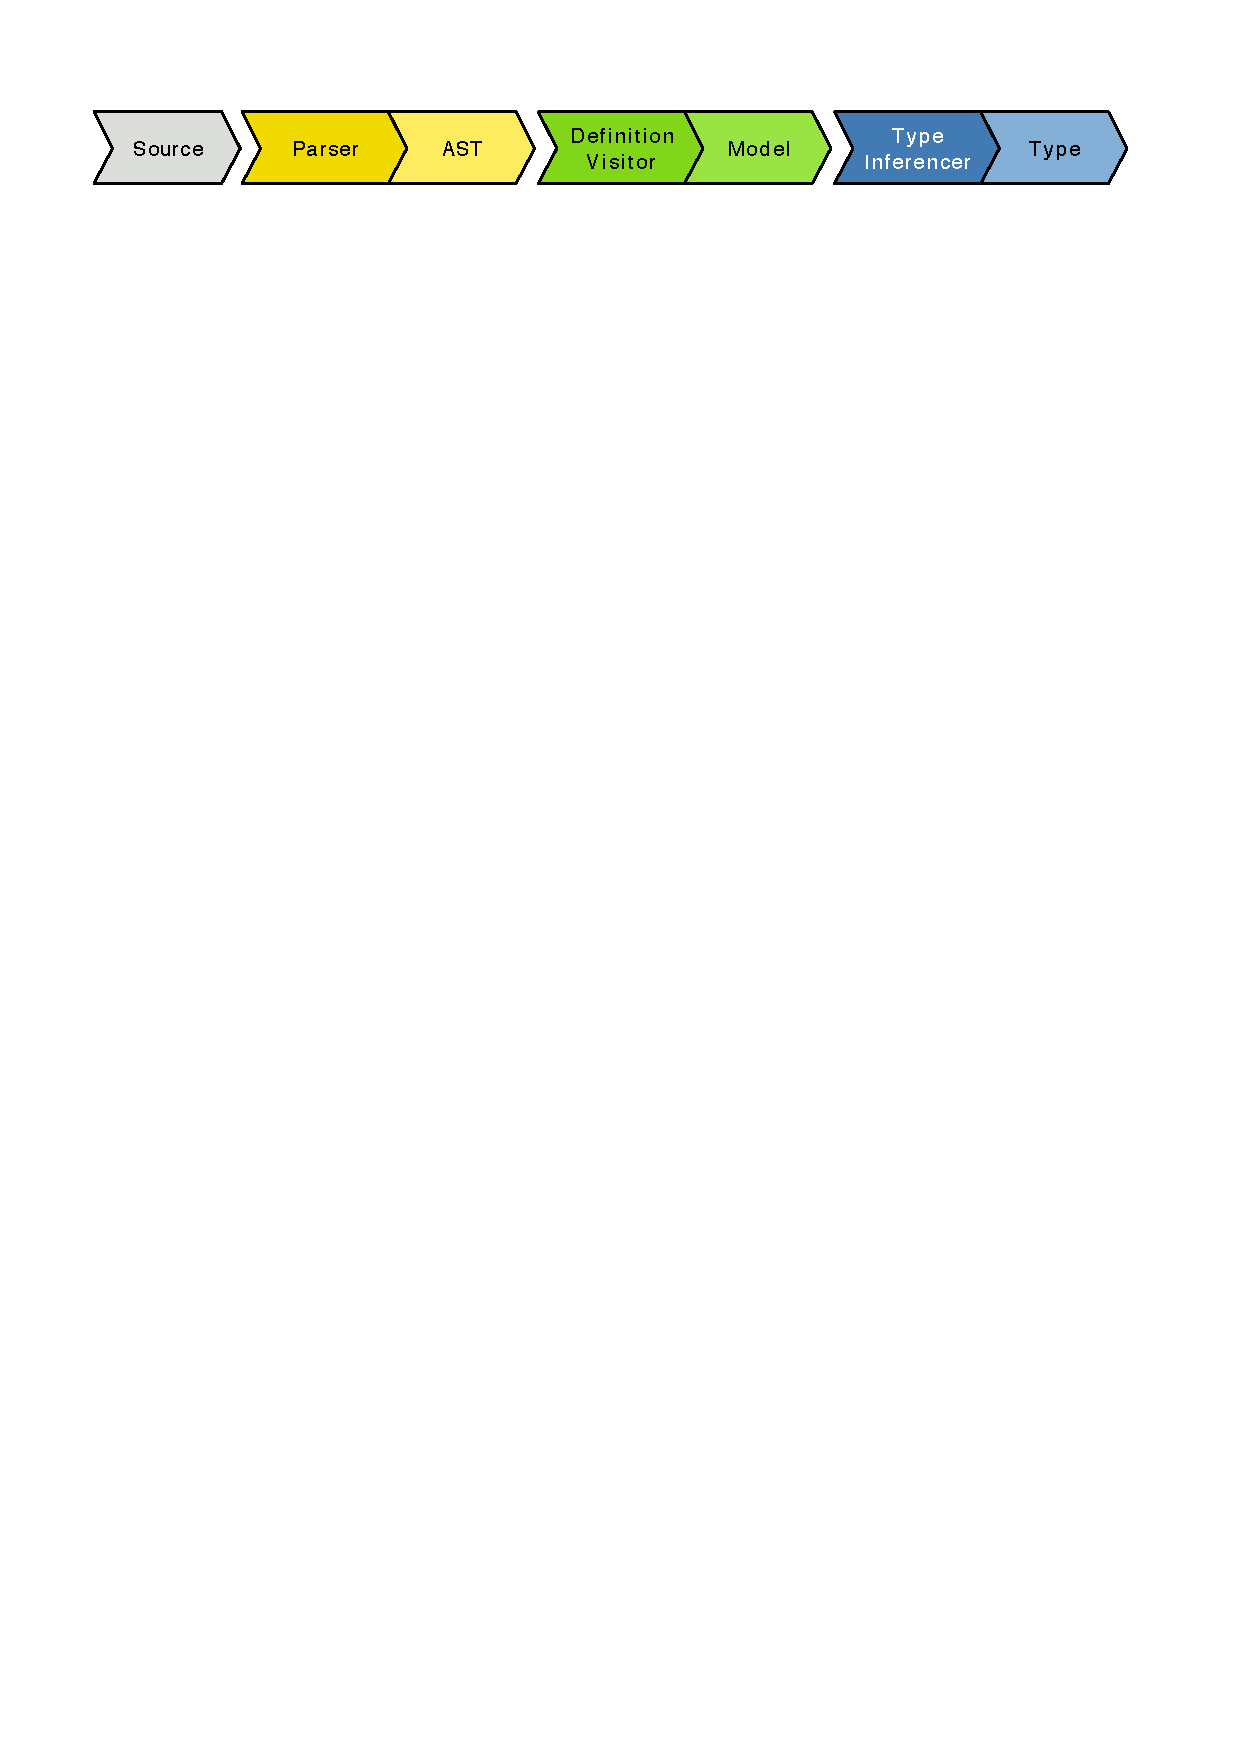
\includegraphics[width=1 \textwidth]{process_overview}
 \label{fig:process_overview}
\end{figure}

The first two steps, the parsing of source code and generation of the model, lay the foundation for the type inferencer. They do a static analysis of the whole project and are independent of???from expr.... what expressions should be evaluated. As long as the underlying source code doesn't change???, these preparations can be reused for any number of type inferencer evaluations.

\chapter{Model}

This chapter describes how the foundation for the type inferencer and the structural analysis is built, namely the model.

\section{Parsing the Source Code}

\begin{wrapfigure}{r}{2.5cm}
    \vspace{-0.6cm}
    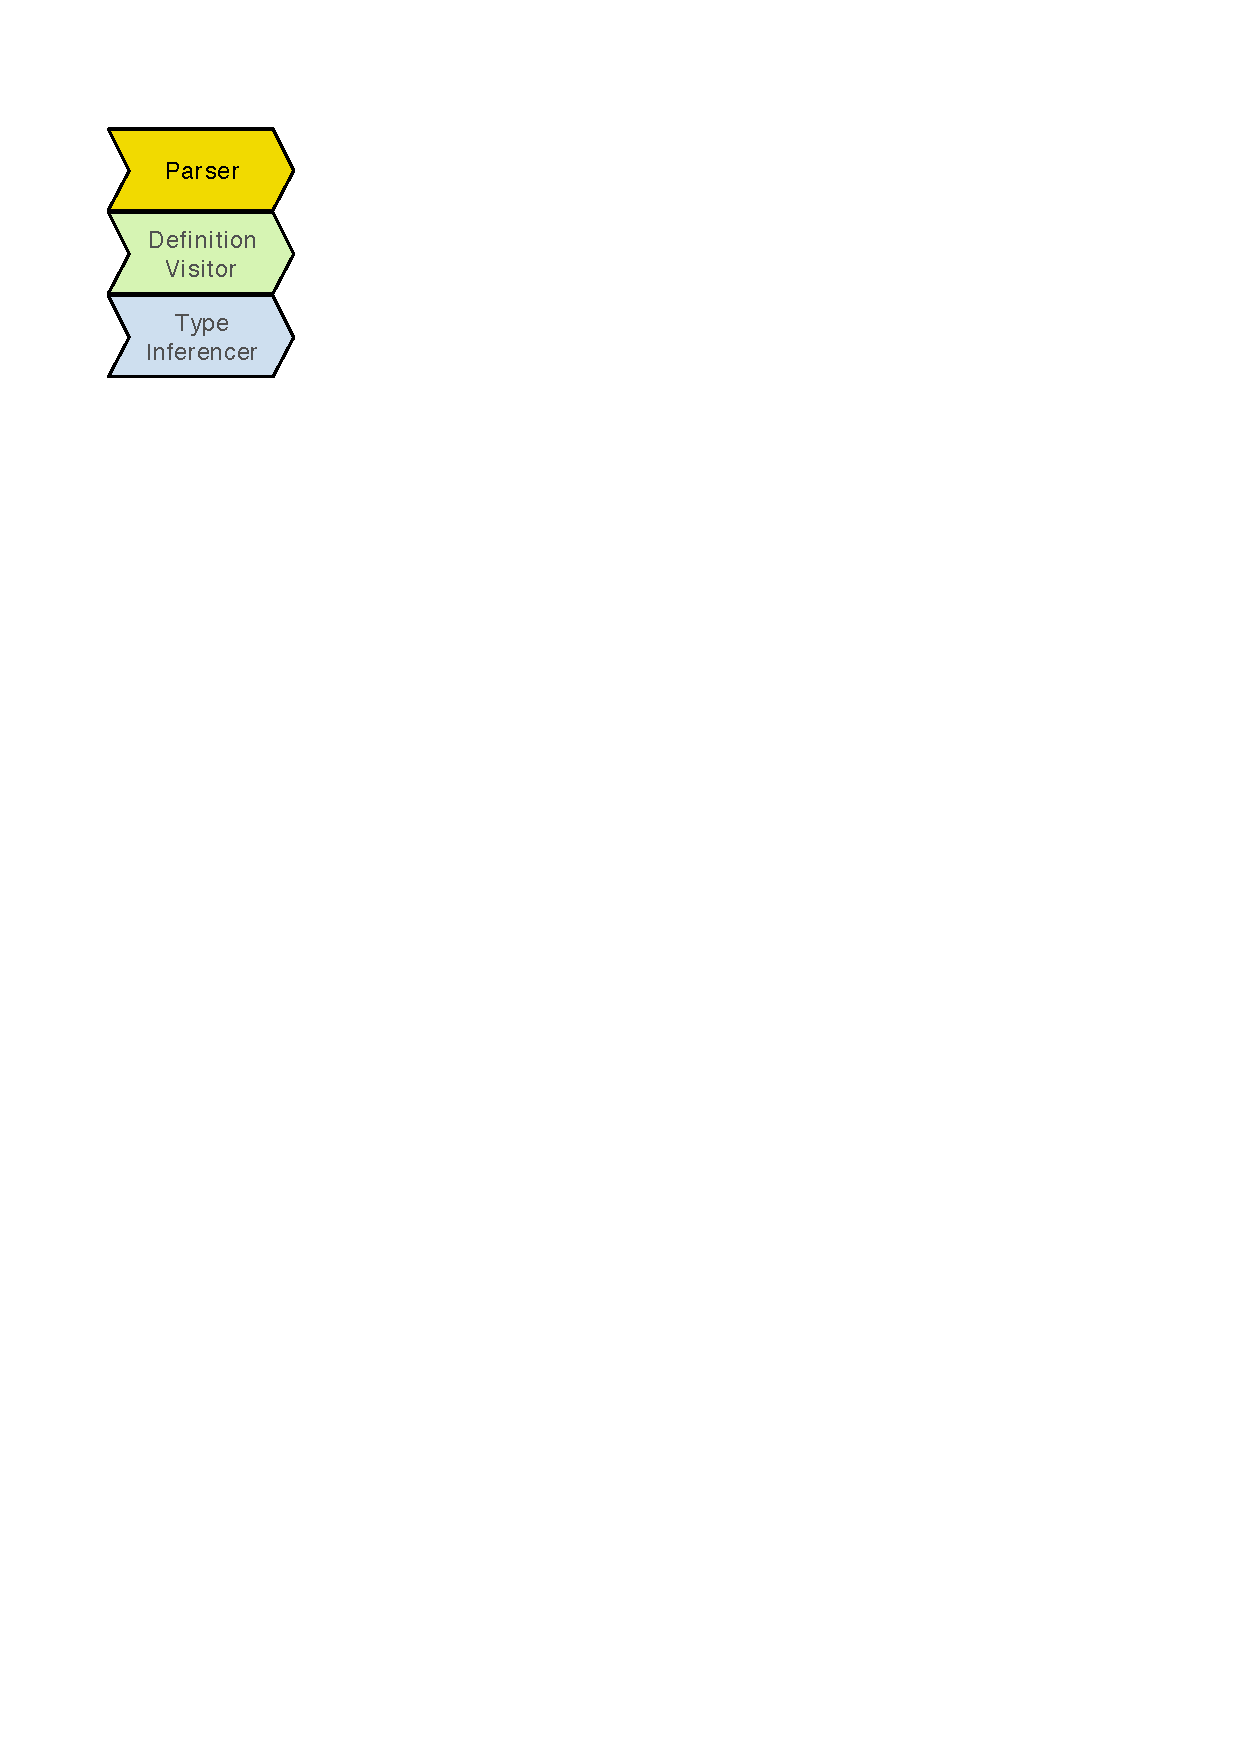
\includegraphics[width=2.5cm]{process_overview_parser}
\end{wrapfigure}

Before any analysis can be done on the application???, its source code has to be brought into a form which is easier to process for programs. It's quite common to express an application's source code as a tree, where an interior node represents a programming language construct and the children of that node represent meaningful components of the construct. For example the simple code \code{foo("bar")} is a call node with the parameter as a string node attached to it. This node structure is usually called abstract syntax tree (AST).

\begin{lstlisting}
Call
|   func = Name("foo"),
|   args = 
|   |   Str("bar")
\end{lstlisting}

Instead of writing a new parser, PyStructure uses a modified version of the Jython\footnote{Jython is a Python implementation for the JVM written in Java.} parser. The modifications were done by the PyDev\footnote{PyDev is an IDE for Python developers based on Eclipse and written in Java.} project to be able to interpret Python 2.5 source code, the normal Jython parser can only parse source code written for Python 2.2. In the long term it would be advantageous to use the unmodified Jython parser, but before 2.5 syntax is supported this is not really an option.

It should be noted that the parser does not do that???-that much besides converting the source code into a tree representation of the syntax. And this representation is still independent of???from the semantics of the interpreter. For example, the Python interpreter handles the expression \code{a + b} the same as \code{a.__add__(b)}, but???whereas the parser still represents the code as \node{BinOp(a, b, op=Add)} and therefore distinguishes it from literally calling the \code{__add__} method, which would be \node{Call(a.__add__, args=b)}.


\section{Creating the Model}
\label{creating_the_model}

\begin{wrapfigure}{r}{2.5cm}
    \vspace{-0.7cm}
    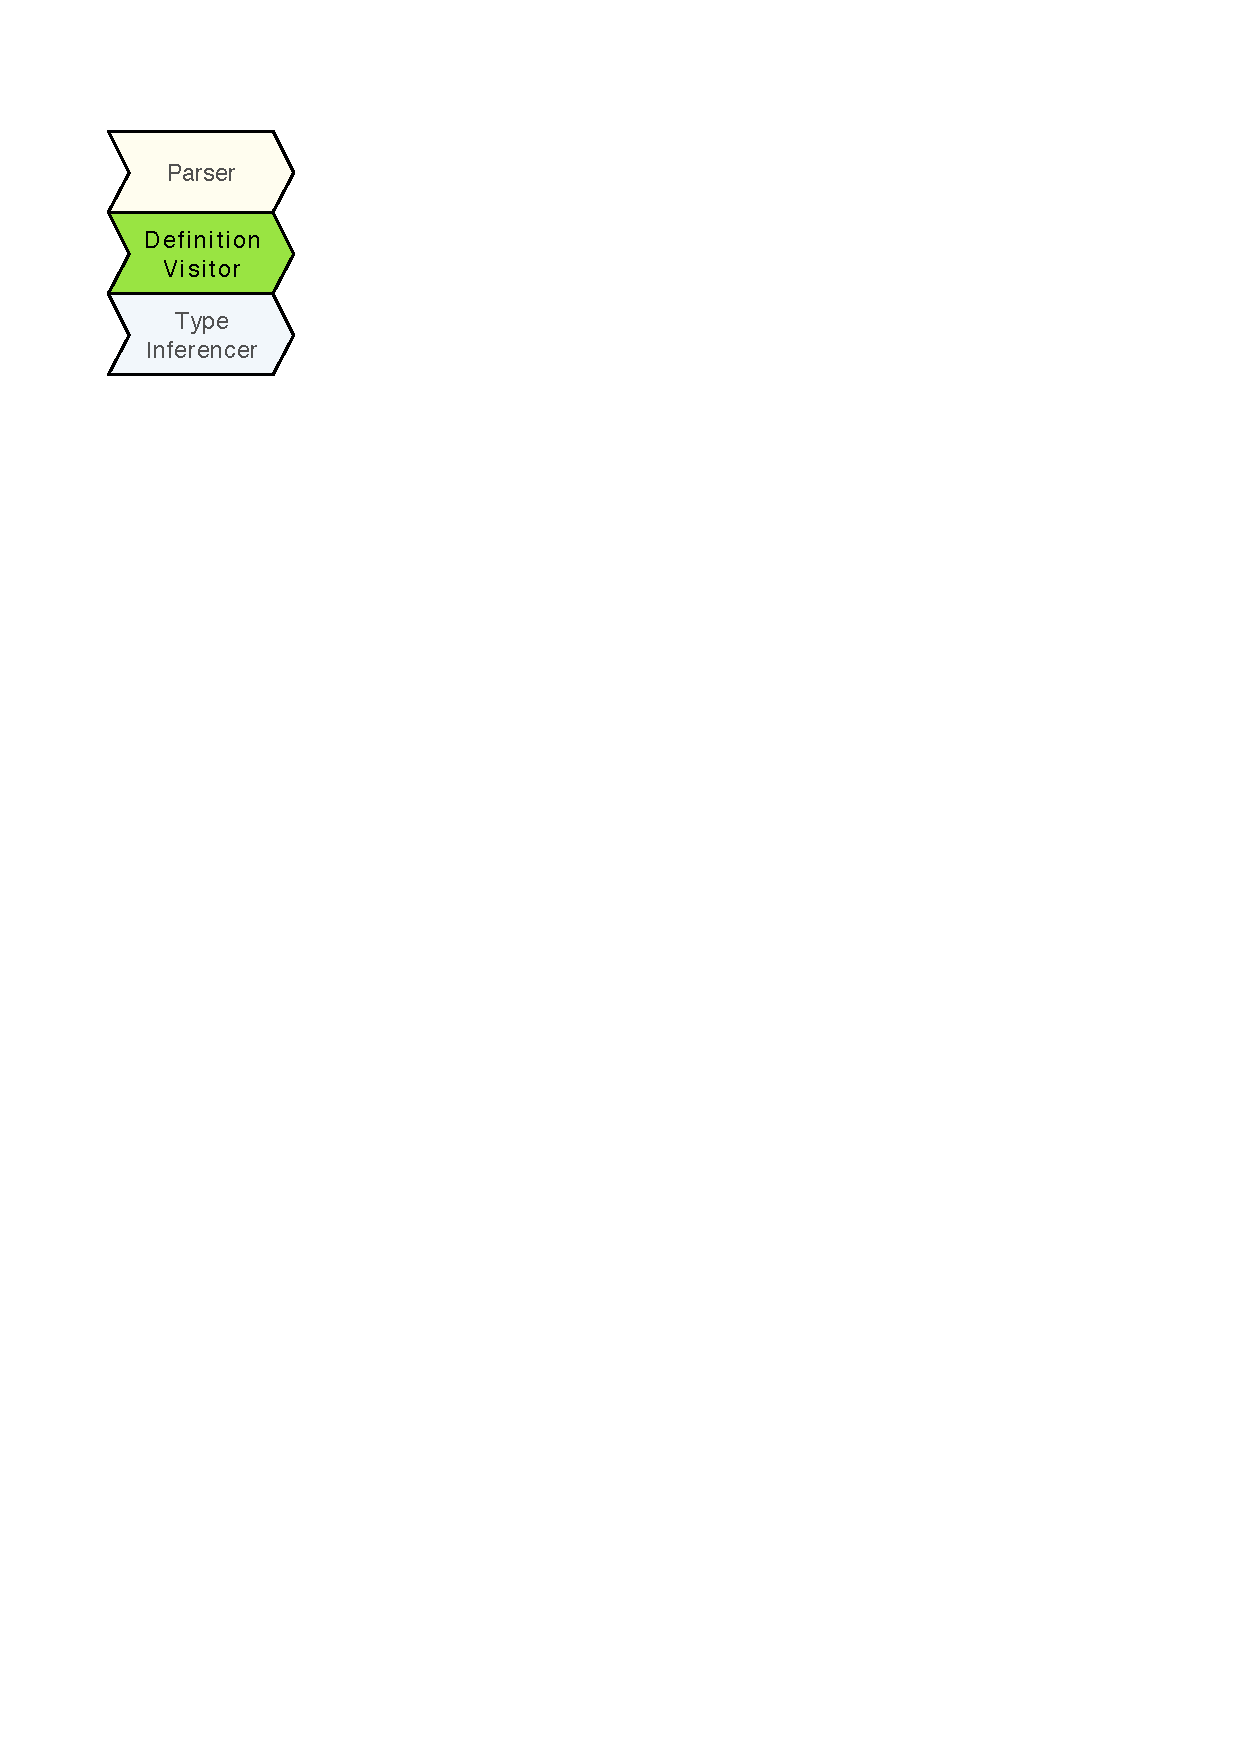
\includegraphics[width=2.5cm]{process_overview_model}
    \vspace{-1cm}
\end{wrapfigure}

The representation of a program provided by the AST is very basic and working directly with it is quite cumbersome. 
One drawback of the AST is that it's just a \emph{syntactical} representation of the source code and doesn't include any semantic information.

For example, in the following code, the AST doesn't know that the two uses of \id{foo} are related:

\begin{lstlisting}
foo = "Hello"
print foo
\end{lstlisting}

They are just represented as two independent \node{Name} nodes in the AST. Also, it isn't easily possible to get all methods of a class without using a visitor every time. Therefore PyStructure uses a second stage in which it processes the AST further. It does some static analysis to create a model which provides a base for the type inferencer to work with. The model consists of the following:

\begin{itemize}
    \item Objects representing the nested structure of the program, such as \class{Module}, \class{Class} or \class{Method}, as well as how they relate to each other, for example \class{Class} knows which methods it contains
    \item Variables and where they are defined and used
\end{itemize}

Types are not yet involved at this stage, the model is just a foundation to make it easier for the type inferencer to do its work. The model is created once and stays the same for all goal evaluations.

\subsection{Creating the Structure}

The first step of???in building the model is to extract the structural elements that make up a program, like modules, classes, methods and functions. These also represent scopes for variables.

Creating this initial structure is done by the structure definition visitor. It is a simple visitor which just visits class and function definitions (method definitions are the same in the AST). Then it creates \class{Class}, \class{Function} and \class{Method} objects, which wrap the AST nodes. They also provide additional functionality, for example the \class{Module} knows which classes and functions it includes and \class{Class} contains methods.

\subsection{Connecting Definitions and Uses}
\label{connecting_definitions_and_uses}

???maybe rewrite this paragraph a bit Now we have the elements of the model, but more is needed. As described in the example with the \id{foo} variable in section \vref{creating_the_model}, knowing the variables where they are defined and used is important for the type inferencer. Determining this is called flow analysis and is based on these two elements:

\begin{itemize}
    \item \textbf{Definition:} Binding of a value to a name, for example through:
    \begin{itemize}
        \item Variable assignment
        \item Class or function definition
        \item Argument declaration
        \item Loop variable declaration
        \item Imports
    \end{itemize}
    \item \textbf{Use:} Reference of a name, for example:
    \begin{itemize}
        \item Variable name
        \item Class or function name
        \item Argument name
    \end{itemize}
\end{itemize}

The task of the flow analyser is to create these elements and connect each use with all its possible definitions.

In the following example, both occurrences of \id{var} on line 1 and 4 are definitions and those on lines 2 and 5 are uses:

\begin{lstlisting}[numbers=left]
var = 42
print var

var = "Hi"
print var
\end{lstlisting}

The two definitions are made unconditionally, which means the two uses each belong to the definition right before them. So the value of the first \id{var} is \code{42}, while the second's is \code{"Hi"}. When an analyser does it this way and respects the flow of the variables, it is called flow-sensitive. If an analyser just takes all assignments to the same name as belonging to the same variable, it is called flow-insensitive.

PyStructure's analyser is flow-sensitive. The advantage is that it results in better precision for inferring types and it is also a very useful feature to have for the use case of an IDE, where it helps with certain refactorings. Unfortunately, a flow-sensitive analyser is more difficult to implement. The following examples show some tricky situations and how the analyser should resolve them.

\subsubsection{Branches}

When conditional assignments are involved, it is more difficult to clearly say which type a variable is of:

\begin{lstlisting}
if sometimes_true():
    x = 42
    print x
else:
    x = 3.14
    print x
print x
\end{lstlisting}

At the first \code{print} statement, \id{x} belongs to the assignment with \code{42}. At the second, it is connected with the assignment above it of \code{3.14}. At the \code{print} statement after the if/else block, both definitions are possible, because which branch is executed is only known at runtime and can't be determined by the analyser. 

Therefore the use has to be connected to both definitions.

\subsubsection{Scopes}

If a variable from an outer scope is read, it isn't possible to specifically determine its type, because that depends on where the variable was assigned:

\begin{lstlisting}
def func():
    print g

g = 1
func()

g = 3.14
func()
\end{lstlisting}

The two calls of \id{func} will print different values, because the outer variable \id{g} is accessed after it has been assigned another value. 

In the function itself, it's not possible to say which definition belongs to the use of \id{g}, so both are connected.

\subsubsection{Global Variables}

Global variables complicate the flow analysis, because they can be assigned from anywhere:

\begin{lstlisting}
g = 1

def func():
    global g
    g = 3.14

print g
func()
print g
\end{lstlisting}

Between the two \id{print} statements, the variable \id{g} was assigned another value from within \id{func}. 

Therefore, the variable \id{g} in the global scope is linked to both definitions.

\subsubsection{Implementation}

Flow analysis as shown above is primarily implemented in one visitor, the \class{DefinitionVisitor}. It visits the AST and creates \emph{definitions} and \emph{uses} of names. Each use can have multiple possible definitions associated with it, and each definitions???-s can belong to multiple uses. In other words, they have a many-to-many relationship.

To resolve the definition of a name, the visitor uses a structure of nested blocks and scopes. Scopes are introduced by class and function definitions, and there's also a scope for the module the code is in. Blocks correspond to lines of code which are usually grouped by indentation.\footnote{Python actually makes indentation even mandatory and therefore doesn't need block delimiters like curly braces or end statements.} Scopes are blocks too, just with special behaviour. The following example is used to explain the algorithm:

\begin{lstlisting}[numbers=left]
x = "unrelated"
print x

def func():
    x = 1
    if random():
        y = 42
        print x
    else:
        y = 3.14
        print y
    print y

func()
\end{lstlisting}

The first line defines a variable with the name \id{x}, the second is a use of this definition.

On line 4, there's a function definition with the name \id{func}. It introduces a scope for the function. Because variables from the whole outer scope could be used from within the function, the visiting of the function body is deferred to later.

Line 14 is a name use of \id{func}. That it is a function call doesn't matter for the \class{DefinitionVisitor}.???sounds a bit weird. moreover, does l14 belong here? is it in order of procession?

The visitor now visits the body of the function. The scope of the function is created, with the module scope as the parent scope. At line 5, there's a definition of the name \id{x}.

At line 7, a block starts for the if clause and there's a definition for \id{y}. Line 8 uses the \id{x} variable. To find the corresponding definition(s), the enclosing blocks is searched for the current definition of \id{x}. So the definition from line 5 is found and the use associated with it.

At line 10, the else clause begins. There's another definition of \id{y} here. Line 11 uses \id{y} and its definition is found directly in the block.

On line 12, the two blocks of the if ???clause have ended. The definitions of both blocks are now set as the current definitions of \id{y}, they are said to flow out from the block. So the use on this line may refer to both???, the definitions in the if/else block and the use is created accordingly.

Now the visitor is finished and can return the name uses and definitions.

\section{Model Overview}

After building the structure and connecting definitions and uses, the building of the model is finished. The components making up the model are:

\begin{figure}[H]
    \centering
    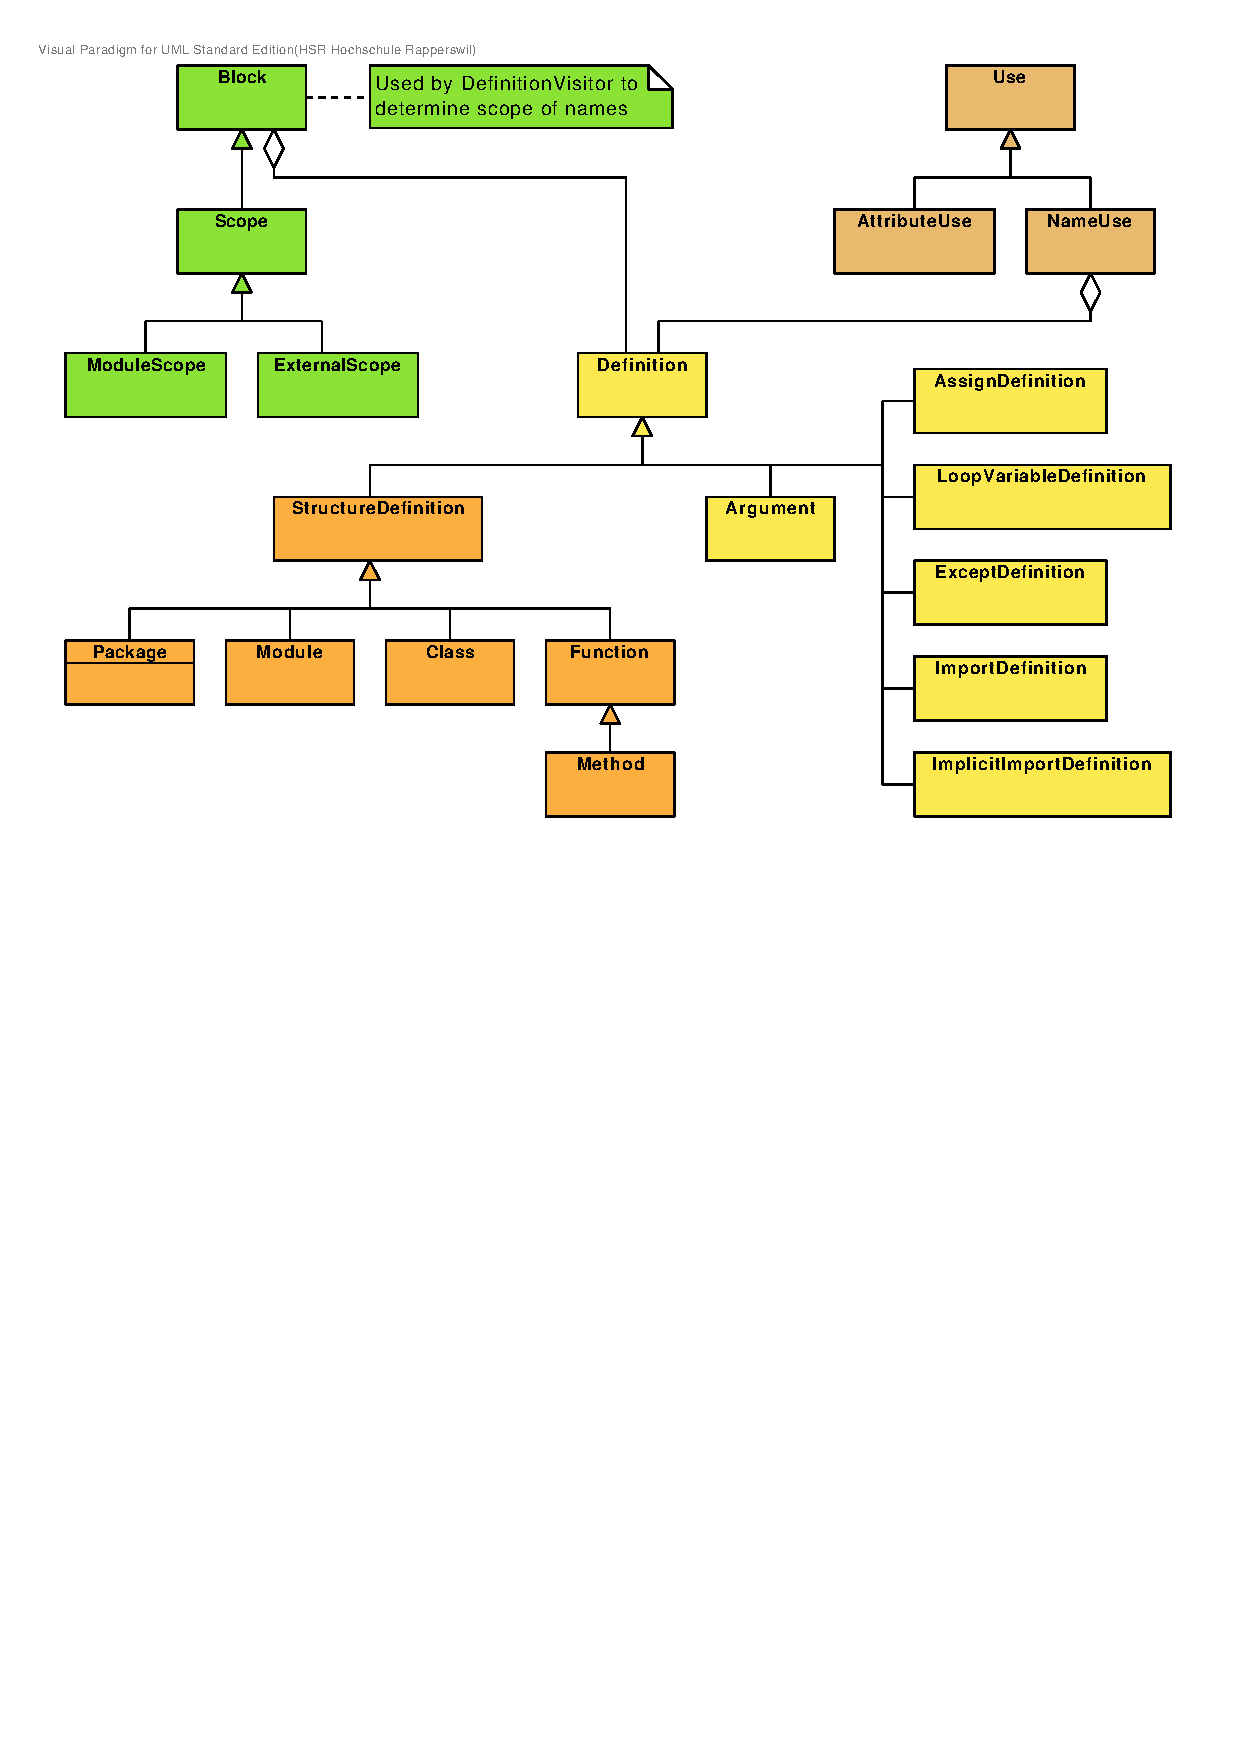
\includegraphics[width=0.8 \textwidth, trim=30 440 30 30, clip=true]{model}
    \caption{Domain Model}
    \label{fig:model}
\end{figure}

\section{Limits of the Model}

There are things which are not represented in the model because it is built without using type inference. Some of these things are:

\begin{itemize}
    \item Which data attributes a class has isn't known, because they are not declared anywhere, they are just assigned as needed.
    \item The class hierarchy can't be resolved during the creation of the model, because the specification of the base class is just an expression and could be the result of a function call or an imported class.\footnote{
    For example: \code{class Foo(calculate_baseclass()): pass}. Of course this kind of class definition is not seen that often.}
    % TODO: do a reference to the MRO C3 section
    \item What exactly is being imported by an import statement.
    \item The model is based on the AST nodes, which means that there may still be multiple ways an operation is represented. For example, \code{x + y} is the same as \code{x.__add__(y)} from a type inference perspective. Therefore these variants have to be handled in the type inferencer.
    % TODO: reference section in outlook/results about transformation of AST to AAST
\end{itemize}


\chapter{Type Inference}

\begin{wrapfigure}{r}{2.5cm}
    \vspace{-0.6cm}
    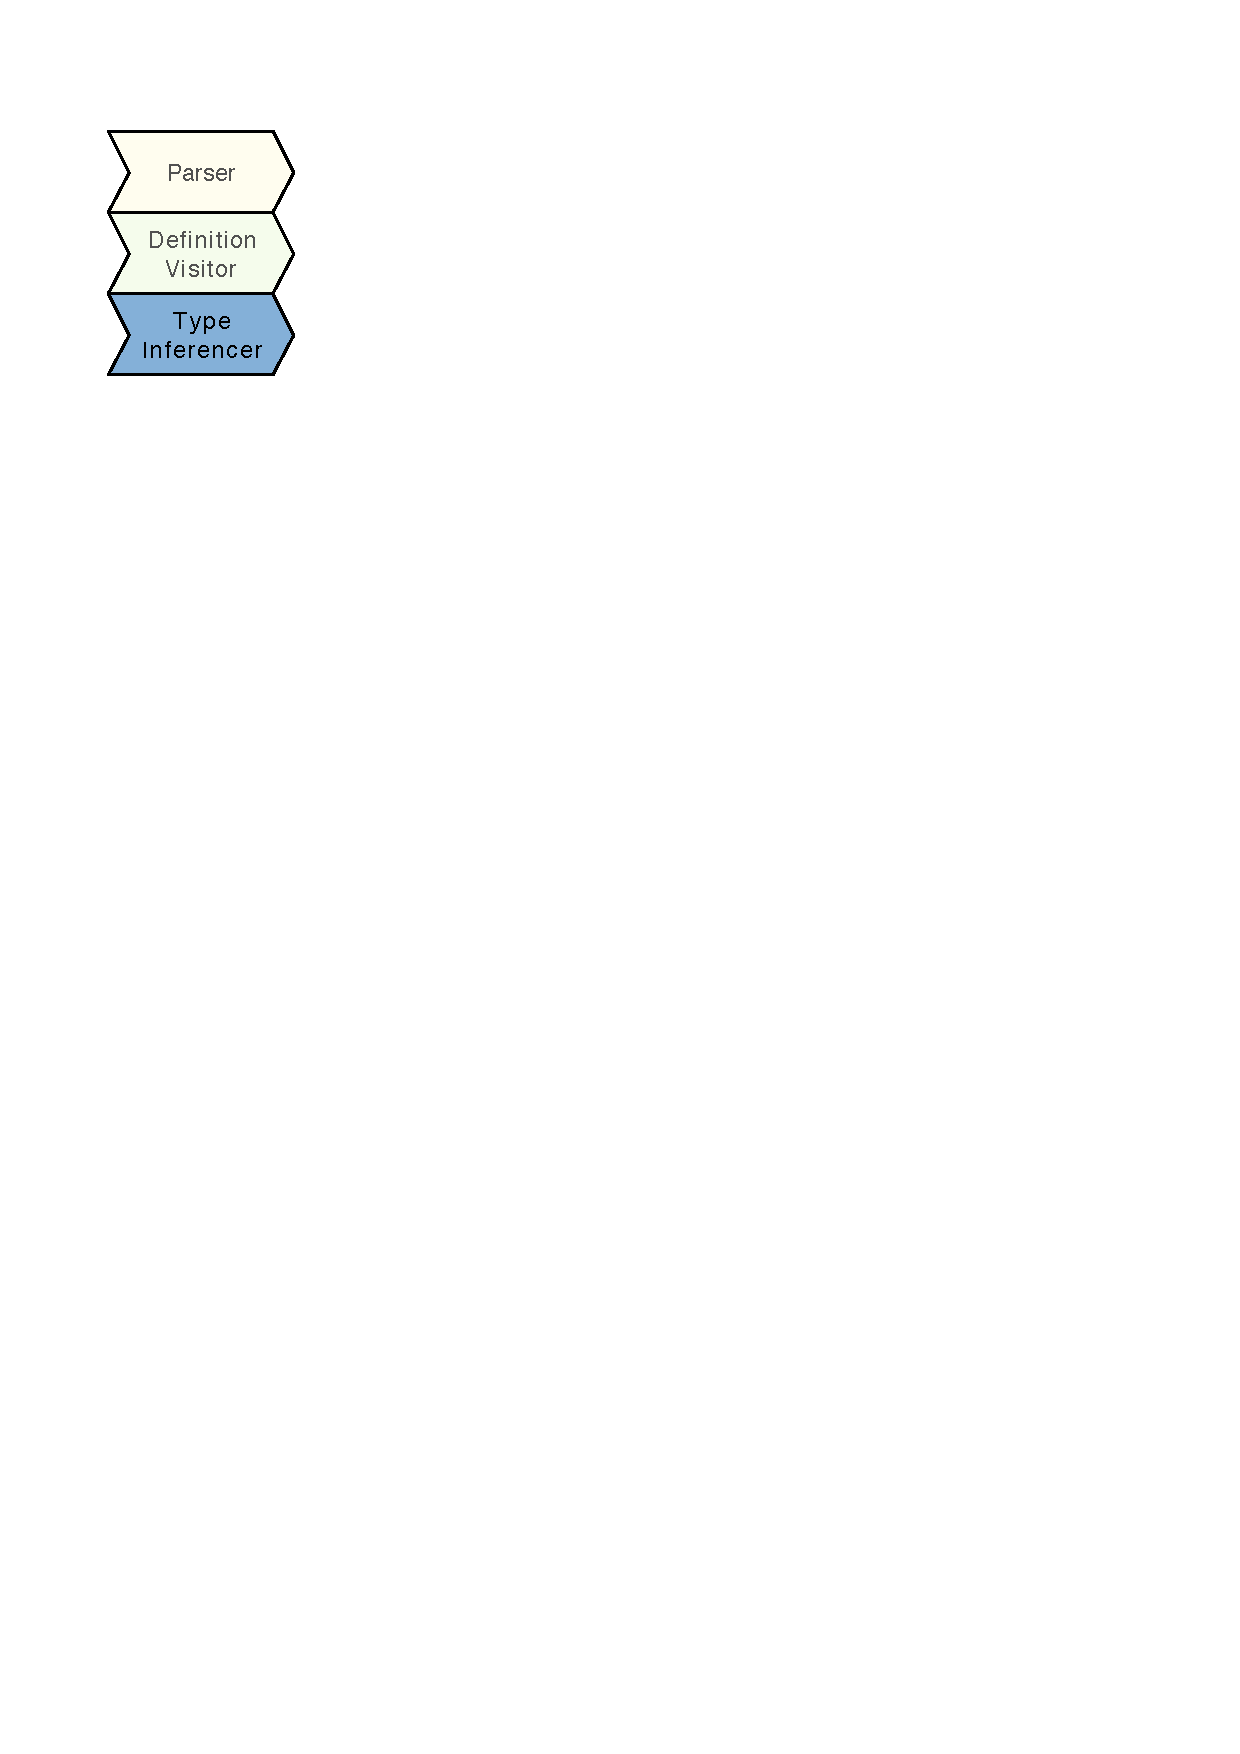
\includegraphics[width=2.5cm]{process_overview_ti}
\end{wrapfigure}

Now, after all the source has been parsed and a generalised model of the program has been built the actual analysis can begin. 

In the first part of this section the \textbf{goal engine} and the general \textbf{evaluation} is described. Knowing how these underlying mechanisms work is important to understand the type inferencer itself. In the second chapter the \textbf{type inference algorithm} itself is explained using some examples. 

\section{Goal Engine}

% (advantages/disadvantages)\\
% (contexts)\\

The goal engine is a central part of the type inferencer, it is???-, it is responsible for the orchestration of the whole evaluation and the underlying algorithm. To understand how the type inference algorithm works it is important to understand the goal engine. Theoretically the goal engine could be used to solve any type of goals.

\subsection{Components}

The goal engine consists of the following main components:

\subsubsection{Goals}

Goals, as the name says, defines the \emph{goal} of a single step in the type inferencer. Usually a goal can't be solved directly, but requires several subgoals to reach a conclusion. ???singular / plural mixup or is goals a common expression?

When a goal is solved the result is stored in the goal object and returned to the evaluator that created it. ???same statement can be found again after the 'examples' -> eliminate one

Examples:

\begin{itemize}
    \item ``What does this function return?''  $\rightarrow$  \class{ReturnTypeGoal}
    \item ``What is the type of this definition?'' $\rightarrow$ \class{DefinitionTypeGoal}
    \item ``Where is this method called?'' $\rightarrow$ \class{MethodReferenceGoal}
\end{itemize}

\subsubsection{Results}

% { rstocker  neuer abschnitt

When a goal gets solved the result is stored within the goal. How this result does look like depends on the kind of goals. 

In PyStructure there are two main kind of goals (and therefore results):

\paragraph{Types}

Report what kind of type a given expression has. There is a distinction drawn between different kind of types. These are:

\begin{itemize}
    \item \textbf{Class Type} A particular instance of a class
    \item \textbf{Metaclass Type} A class object
    \item \textbf{Method \& Function Type}
    \item \textbf{Package Type}
    \item \textbf{Combined Type} Union of several types
\end{itemize}

In the example \code{t = Truck()}, \id{Truck} is a Metaclass Type wereas \id{t} is a Class Type.


\begin{figure}[H]
    \centering
    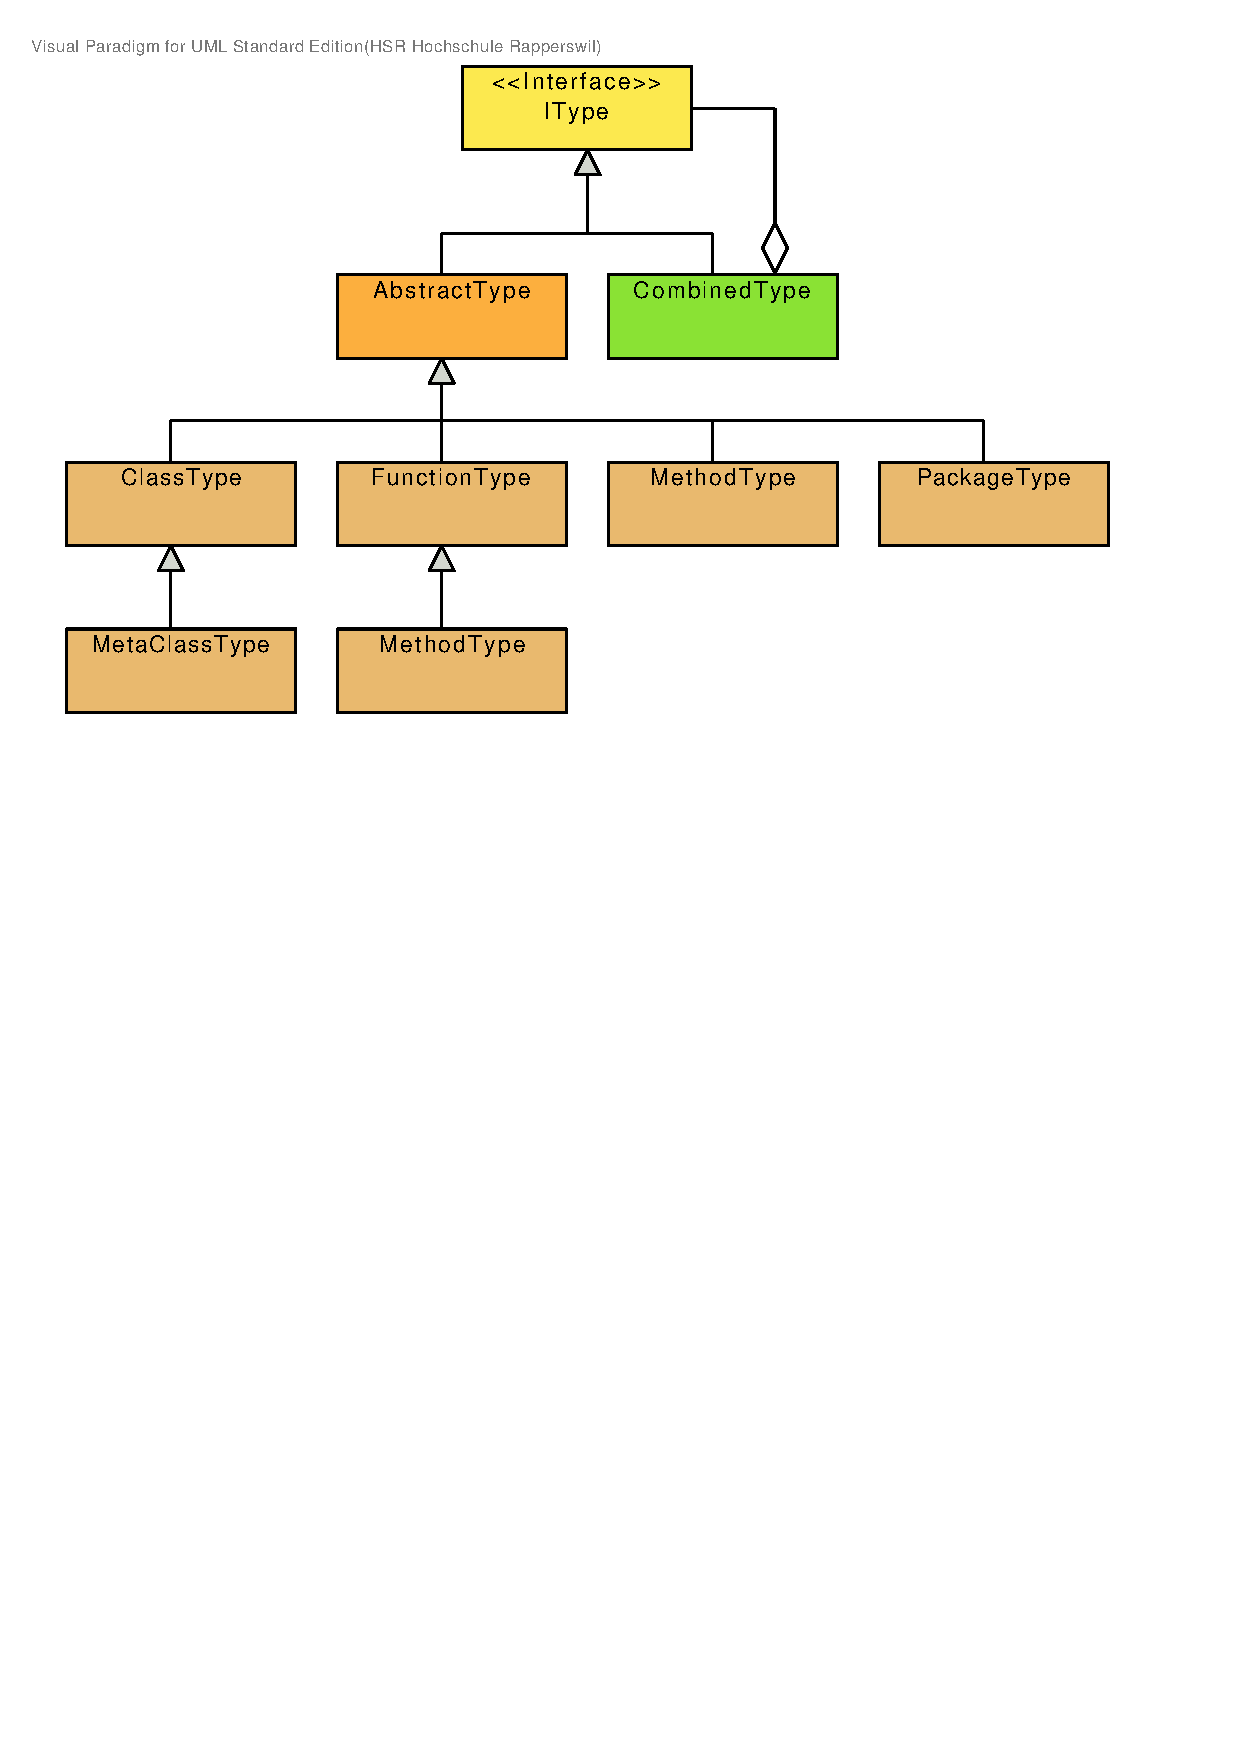
\includegraphics[width=0.8 \textwidth, trim=30 500 60 30, clip=true]{ti_results}
    \caption{Domain of the result types}
    \label{fig:ti_results}
\end{figure}

\paragraph{References}

Some goals return a list of references when being solved. As explained later this is for example used when the type infer???-infer inferencer has to find all callers of a given method.

Several kinds of references are used:

\begin{itemize}
	\item Attribute References
	\item Class References
	\item Function References
	\item Method References
	\item Constructor References
\end{itemize}


\begin{figure}[H]
    \centering
    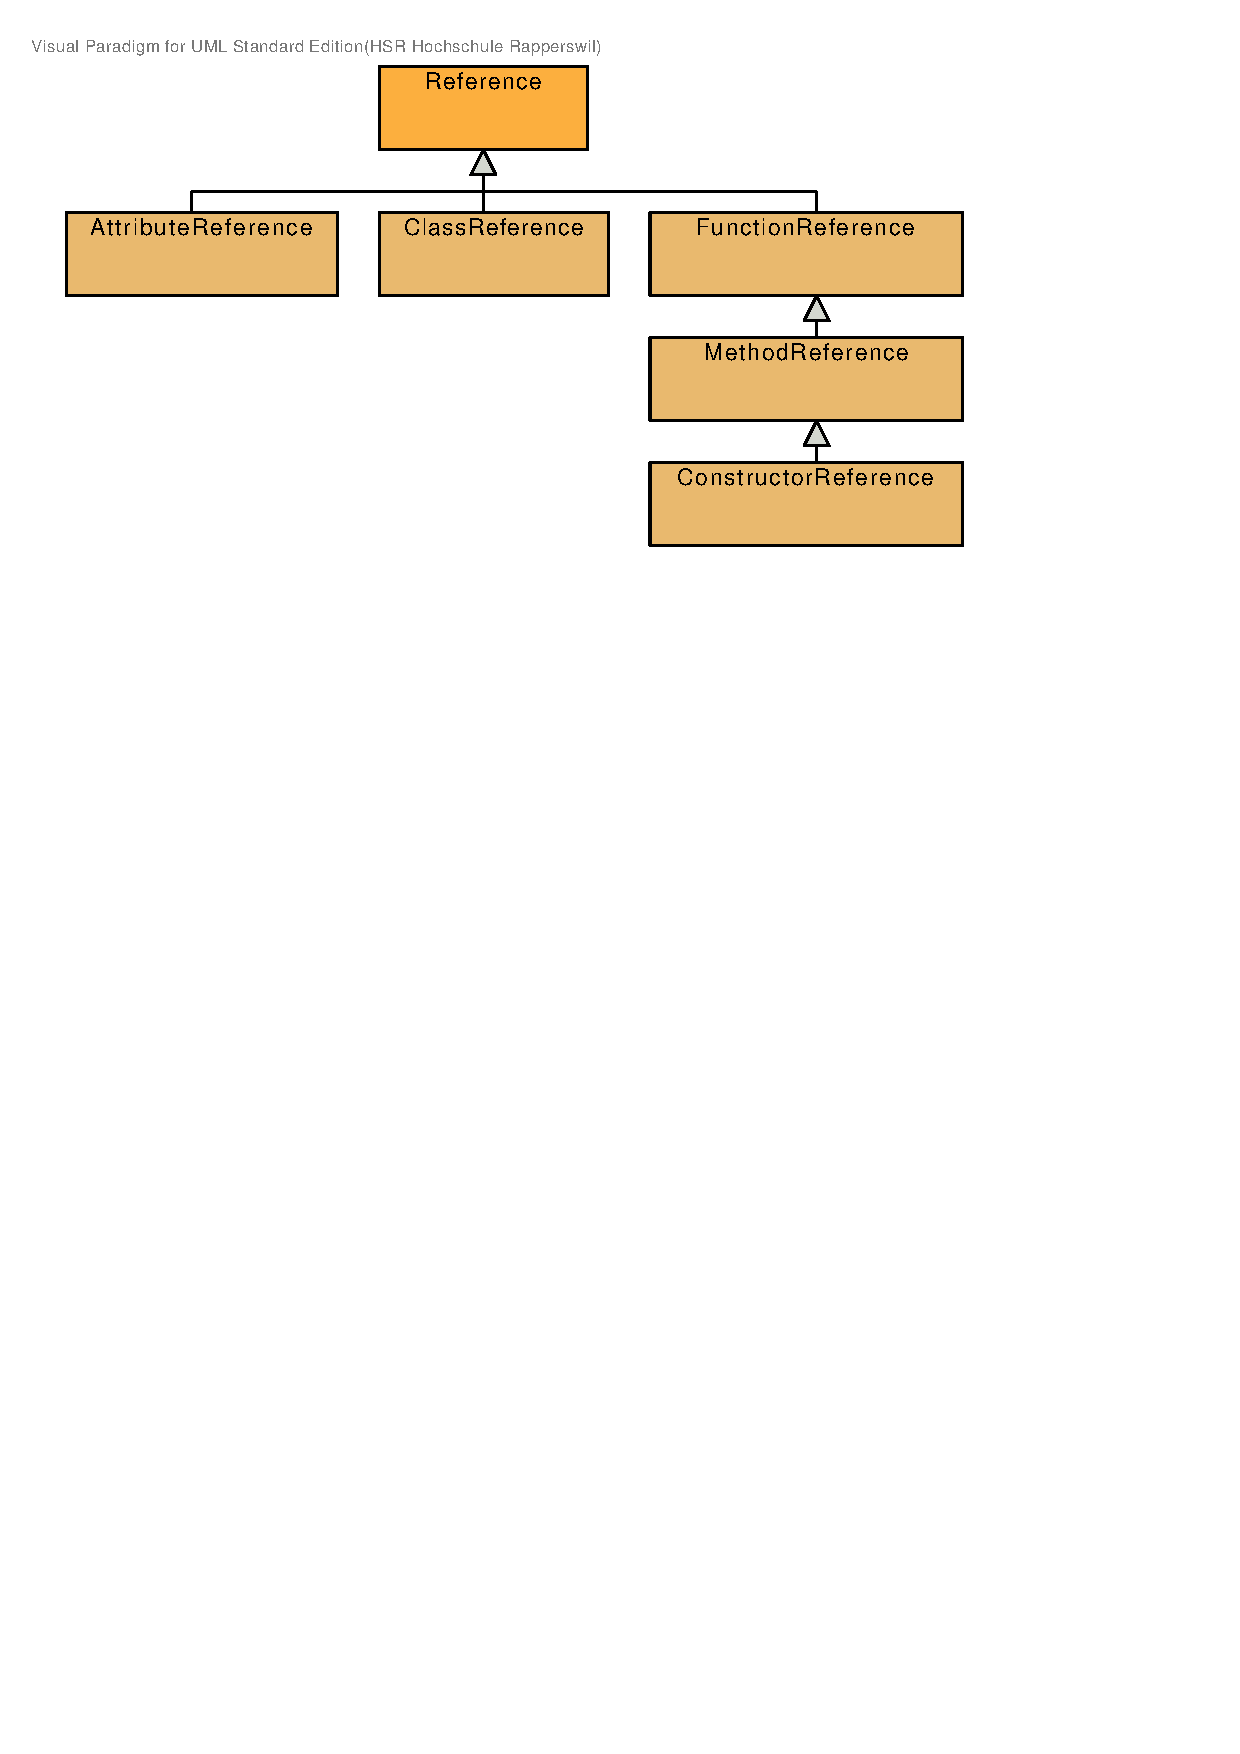
\includegraphics[width=0.7 \textwidth, trim=30 530 125 30, clip=true]{ti_references}
    \caption{Domain Model of the reference types}
    \label{fig:ti_referenes}
\end{figure}

% }

\subsubsection{Evaluators}

The counterpart of the goals are the evaluators, which are responsible for solving a particular goal. If they need any further information they can create subgoals. The evaluator is notified when a subgoal is finished???finishes. 

\subsubsection{Evaluator Factory}

The final part which brings goals and the???-the evaluators together is the evaluator factory. It is responsible for choosing the right evaluator for a particular goal.???now i get it with the counterpart :)

\subsubsection{Goal Queue}

Internally the goal engine basically keeps goal nodes in a working queue. A goal node combines a goal and its evaluator. The algorithm works like in this simplified pseudocode:

\begin{lstlisting}
def evaluate_goal(root_goal):
    queue = []
    add_goal(queue, root_goal)

    while len(queue) != 0:
        goal_node = queue.pop_front()

        if goal_node.is_new():
            subgoals = goal_node.init()
            add_goals(queue, subgoals)

        if goal_node.is_done():
            goal_node.finish()
            for parent in goal_node.parents:
                subgoals = parent.subgoal_done(goal_node)
                add_goals(queue, subgoals)
        else:
            queue.append(goal_node)
\end{lstlisting}

A goal is done when all its subgoals are done or when it created no subgoals in the first place. The \id{add_goals} method takes some measures to prevent the goal engine from running without ever stopping, see section \vref{recursion}.

Each goal node knows all its parent goal nodes, which will be notified with the result when its evaluation is done. All the goal nodes form a graph, to be specific a directed acyclic graph (DAG).

\todo{describe some goal engine behaviors like, cyclic recursion, caching, crazy ordering and so on}



\subsection{Evaluation Process}

Summarised, the evaluation works as follows: First a???-a an expression of interest has to be chosen somewhere in the code. The expression is then attached to an ``expression type goal''. This goal, called root goal because it is the root of the evaluation, is then fed into the goal engine which starts to process it. Every goal has to be processed by one evaluator. Which evaluator has to be used is determined by the evaluator factory according to the goal's type and other criteria. The particular evaluator is then initialised and processes the goal. The evaluator can (and usually will) create subgoals which are then processed as well. As a goal finishes successfully, its result is reported back to the parent goal. As soon as the root goal finishes, the result is returned to the user.

\subsubsection{Picking a Root Goal}

As a first step the user of the type inferencer, usually the structural analyser, has to define what has to be evaluated. This \emph{main} goal is called root goal. Usually this goal is an \class{ExpressionTypeGoal} which instructs the goal engine to determine the type of a given expression (hence the name). The expression in question can be any expression from the AST. They can for example be selected using a visitor like the \class{ExpressionAtLineVisitor} or by iterating over all expressions (like the type spider does \todo{reference to the Spider}).

\subsubsection{Selecting the Evaluator for a Goal}

When the root goal is created it has to be fed into the goal engine. Every goal has to be processed by one of the available evaluators. Which one has to be used is determined by \class{PythonEvaluatorFactory}.

The \class{PythonEvaluatorFactory} takes several criteria into account. In the case of an expression type goal the type of the associated expression is also considered. For example if the expression is a method call the goal is delegated to the \class{CallTypeEvaluator}, an attribute expression (e.g. \code{obj.method}) is processed by the \class{AttributeTypeEvaluator} and so on.\todo{rstocker: Should we a provide a list of these mappings somewhere?}

\subsubsection{Evaluator}

Now the actual work begins, the evaluator is created with its goal as a parameter. As a first step the eveluator's \java{init()} method is called. The evaluator then has a first chance to do it's job. If necessary (and it often is) the evaluator can create subgoals and return them. The evaluator's goal is not considered finished as long as there are remaining unfinished subgoals. Every time a subgoal is finished the evaluator's \java{subgoalDone(subgoal)} method is called. Here again the evaluator has the chance to create more subgoals as needed.

From the goal engine's perspective there's no difference between subgoals and root goals, they are handled equally. But of course as soon as the root goal is finished the goal engine returns the calculated result to the user.
    
\section{Type Inference Algorithm}

The implementation of the type inference algorithm consists of the goal engine and \textbf{15 goals} and \textbf{31 evaluators}.

The internal workings of the type inferencer are best described using some examples. In this section some common situations are shown and it is explained how the type inferencer solves them.

It is important to understand that all goals of the examples can be mixed and matched freely. Although these examples look unrealistically simple, they can be combined in whatever order is necessary, and therefore catch a lot of different and complex cases.


\subsection{Simple Assignment}

The first example is quite simple, a new object of the class \id{Foo} is instantiated and assigned to the variable \id{x}. 

\begin{lstlisting}
class Foo(object):
    pass

x = Foo()
x # what type?
\end{lstlisting}

\begin{itemize}
    \item The type inferencer is initialised with an \class{ExpressionTypeGoal} with the node \node{Name(x)} associated to it.
    \item The evaluator factory looks at the goal and creates an \class{NameTypeEvaluator} for it because the expression in question is a Name AST node.
    \item The \class{NameTypeEvaluator} finds the definition of \id{x} by looking for the corresponding \class{NameUse} in the module. It then creates a \class{DefinitionTypeGoal} to determine its type. Note: if there is more than one definition the evaluator just creates a subgoal for each of them. \todo{we could mention somewhere that this easy parallelising a advantage of the goal engine is}
    \item In this case the node attached to the definition is an \node{Assign} node and therefore the goal is mapped to the \class{AssignTypeEvaluator}.
    \item All the \class{AssignTypeEvaluator} does is creating a new \class{ExpressionTypeGoal} for the corresponding value on the right-hand side of the assignment. In this case this is: \code{Foo()}.
    \item Note: As \id{Foo} is capitalised it is quite obvious for the human observer that we are talking about the instantiation of an object here. But Python allows capitalised function names and therefore the TI can't be completely sure and therefore has to check what \id{Foo} actually is, a function or a class.
    \item This new \class{ExpressionTypeGoal} is also processed by the evaluator factory, but this time a \class{CallTypeEvaluator} is created as the goal's expression is a \node{Call} node: \code{Foo()}.
    \item The evaluator first tries to determine if the name in question is a function or a class. To do that it creates an expression type goal for the name. In this case this is the name \id{Foo}.
    \item Now the type of the name \id{Foo} has to be evaluated, which works like with the \id{x} name at the beginning. The \class{NameTypeEvaluator} finds the class definition, and the returned result is a \class{MetaclassType}.
    \item The result is handed back to the \class{CallTypeEvaluator} which now knows that the call is in fact a constructor, so therefore the type returned by the call is an object of the class \class{Foo}, which is a \class{ClassType}.
    \item Not much is left to do. The final result is handed up the chain of evaluators until the evaluator of the root goal is reached, the first \class{NameTypeEvaluator}.
    \item After the root goal is finished the result is handed back to the caller of the library and the type inference process is finished.
\end{itemize}

So, briefly summarised the evaluation works as follows: First the TI locates the variable's definition, in this case an assignment and then finds out what was assigned.

\subsection{Function Call}

The second example is similar to the first one, but instead of the creation of a new object a function is called.

\begin{lstlisting}
class Bar():
    pass

def function():
    return Bar()

x = function()
x # what type?
\end{lstlisting}

\begin{itemize}
    \item The first few steps are similar to the first example, the evaluator eventually creates an \class{ExpressionTypeGoal} for the expression \code{function()}.
    \item Because it is a \node{Call} node as above, a \class{CallTypeEvaluator} is used again. And as in the last example the name of the function being called is resolved: \id{function}.
    \item The name \id{function} leads to the function definition and is returned to the \class{CallTypeEvaluator}.
    \item Now knowing that it's a function the evaluator creates a \class{ReturnTypeGoal} for it.
    \item The \class{ReturnTypeGoal} is handled by the \class{ReturnTypeEvaluator}, which creates an \class{ExpressionTypeGoal} for every return statement in the function.
    \item[$\rightarrow$] In this case the result of a \code{Bar()} call is returned.
    \item From this point on the evaluation continues like in the previous example.
\end{itemize}

So the only difference between creating an object and calling a function is that for the function, all the return statements have to be analysed.

\subsection{Arguments}

The next example shows a different important problem: How are the types of arguments found. To determine these it isn't sufficient to know only the definition, all callers of the function have to be known as well

\begin{lstlisting}
class Baz():
    pass

def function(arg):
    x = arg
    x # what is x
    
function(Baz())
\end{lstlisting}

\begin{itemize}
    \item Again the beginning is quite similar to the previous examples, \id{x} is assigned \id{arg}. And \id{arg} is defined in an \node{Argument} node. The \class{DefinitionTypeGoal} for it is therefore passed to an \class{ArgumentTypeEvaluator}.
    \item First the \class{ArgumentTypeEvaluator} has to find all callers of the function \id{function}. To find these it creates a \class{FunctionReferencesGoal}.
    \item The \class{FunctionReferencesEvaluator} first looks for all potential references by setting up a \class{PossibleReferencesGoal} with the name of the function attached to it.
    \item The \class{PossibleReferencesEvaluator} iterates over all name uses (in all modules) and checks if their name matches the function's. \textbf{} \\\textbf{Note:} \emph{The \class{PossibleReferencesEvaluator} doesn't really care if the name uses found are actually calls or just something else which just happens to be named the same way.}
    \item To find out which one of these potential references are real callers the \class{FunctionReferencesEvaluator} iterates over all of them and for each one creates an \class{ExpressionTypeGoal}.
    \item The expressions get resolved and the \class{FunctionReferencesEvaluator} just keeps the references which point back to the function in question.
    \item Finally with all the callers known the \class{ArgumentTypeEvaluator} can evaluate the types of the passed arguments by creating an \class{ExpressionTypeGoal} for each one.
    \item[] In the example this would just be \code{Baz()}.
\end{itemize}

\subsection{Methods \& Attributes}

Classes added yet another layer of complexity to the type inferencer. Methods calls are in Python written as \code{receiver.method()}. Here again the problem was to find all callers of a method. Like in the case of functions the evaluator has to check all potential matches if their names match. But this isn't enough,  additionally the receiver has to be of the correct type. Otherwise the TI would mix up a identically called method in two unrelated classes. 

Attributes are even worse. Finding all references of an attribute is quite comparable to finding methods. But in Python attributes are nowhere defined, the developer can just use them and they are created ad hoc.???rewrite that prev. sentence Because attributes are public this doesn't haven???-n oder +e :) to be in the module in which the class was defined.

In this example the TI evaluates the type of the truck's attribute cargo.

\begin{lstlisting}
class Stones(object): pass
class Truck():
    def __init__(self):
        self.cargo = None
    
    def load(self, something):
        self.cargo = something

a = Truck()
a.load(Stones())
a.cargo # what's the type?
\end{lstlisting}

\begin{itemize}
    \item The expression being evaluated is in this case: \code{a.cargo}. \\
          \textbf{Note:} \emph{In the AST this is stored as \node{Attribute[value = a, attr = cargo]}}
    \item The \class{AttributeTypeEvaluator} is used for evaluating \node{Attribute} nodes
    \item Evaluating attributes is done in two steps:
    \begin{itemize}
        \item[1.] Evaluate the receiver \\$\rightarrow$ a
        \item[2.] Look for the method/attribute in the type of the receiver \\ $\rightarrow$ Attribute \id{cargo} in type \class{Truck}
    \end{itemize}
    \item[] \textbf{Note:} \emph{The first step was explained in previous examples, so it isn't described again.}
    \item The \class{AttributeTypeEvaluator} learns that \id{a} is a \class{Truck} object. At this point it's still unsure if cargo is a method or a real attribute. To check if it is a method a \class{MethodResolveGoal} is being created.
    \item The \class{MethodResolveGoal} is handled by the \class{MethodResolveEvaluator}. It checks if a method with a given name is in a particular class or its base classes.\\
          In the example \id{cargo} is a attribute and therefore a method can't be found
    \item Because the \class{MethodResolveGoal} was unsuccessful and didn't have a result, the \class{AttributeTypeEvaluator} evaluates if there is a attribute with this name by issuing a \class{ClassAttributeTypeGoal}.
    \item The \class{ClassAttributeTypeEvaluator} starts by creating an {AttributeReferencesGoal} which tries to find all references of a particular attribute.
    \item The \class{AttributeReferencesEvaluator} works in a similar manner as the \class{FunctionReferencesEvaluator} described in the second example:
    \begin{enumerate}
        \item Find all potential references with the \class{PossibleReferencesEvaluator}
        \item Only keep references to \class{AttributUse}
        \item Only keep references whose receiver has the correct type (is a Truck)
    \end{enumerate}
    \item Using these three steps the the attribute reference evaluators returns three results:
    \begin{itemize}
        \item \code{self.cargo = None}
        \item \code{self.cargo = something}
        \item \code{a.cargo}
    \end{itemize}
    \item \textbf{Note:} \emph{\id{self} and \id{a} are all of type \class{Truck}}
    \item Now the \class{ClassAttributeTypeEvaluator} knows all the places where the attribute was references. All what is left do do is to select all references which are used in a assignment (only the first two) and run an \class{ExpressionTypeGoal} on the values of them: \code{None} and \code{something}.
    \item The assignment of \code{None} produces the type \class{NoneType}
    \item The the second assignment of \id{something} is defined as a parameter of the method \id{store}. Resolving this parameter causes a \class{MethodReferenceGoal}, which itself produces yet another \class{AttributeReferencesGoal} to find all callers of the method.

So here again, finding all callers of a method and finding all attribute references is quite similar, and therefore shares a lot of code/goals.
    
\end{itemize}

\section{Challenges/Problems}

In this section, some of the difficult parts of developing a type inference system for Python are described in more detail. Each problem is illustrated with examples and shows the solution which was implemented in PyStructure is explained.???rewrite, 2 verbs

\subsection{Recursion}
\label{recursion}

Recursion is a normal part of programming languages where a function is called from within itself until a certain condition is met and the recursion stops. It is often used for algorithms like the factorial function:

\begin{lstlisting}
def factorial(number):
    if number <= 1:
        return 1
    return number * factorial(number - 1)
\end{lstlisting}

For a naive type inferencer that isn't prepared to handle it, recursion results in an endless loop in the goal engine. An example is the the evaluation of the return type of the \id{factorial} function. The first return value (\code{1}) doesn't cause problems, but the second does. For calculating the type of the second return value, the return type of \id{factorial} is needed again. So another return type evaluator for \id{factorial} is created and the whole story begins anew, resulting in an endless loop.

\subsubsection{Handling Duplicate Goals}

PyStructure's goal engine has a mechanism in place to detect that a goal has already been created. When this is the case, it just connects the already existing goal node with the evaluator which has asked for the same goal. When the existing goal is finished, the result is passed to the evaluator as usual. But does this suffice to prevent endless looping? Let's look at a simpler recursive example to answer that question:

\begin{lstlisting}[numbers=left]
def recursive():
    if sometimes_true():
        return 1
    else:
        return recursive()

recursive() # what type?
\end{lstlisting}

For evaluating line 5, a new return type goal is created, which already existed because of line 7. So the existing return type goal is connected to the evaluator instead of the new one. After this, the goal node graph looks like this:

\begin{figure}[H]
    \centering
    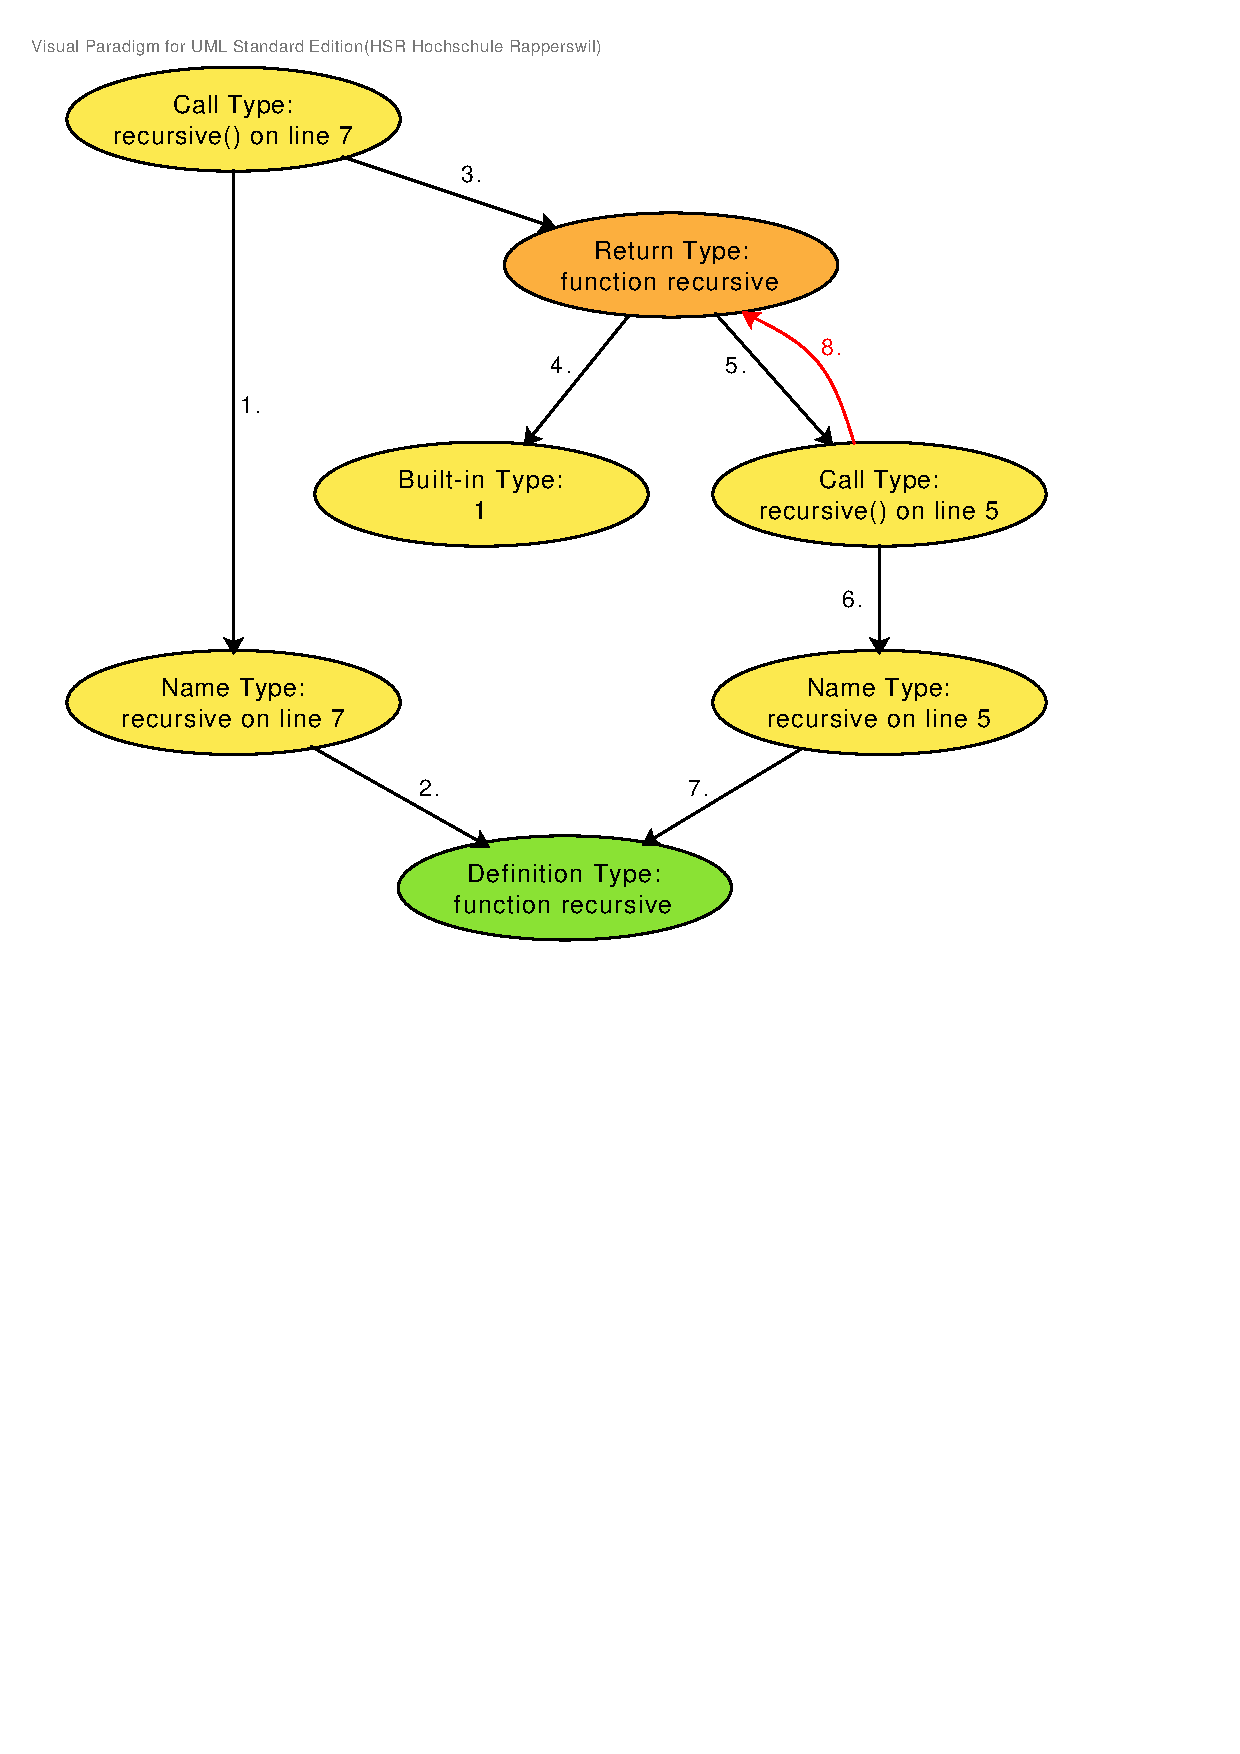
\includegraphics[width=0.7\textwidth, trim=30 380 80 30, clip=true]{recursive_goal}
    \caption{Evaluation with a recursive goal}
    \label{fig:recursive_goal}
\end{figure}

The creation of the call type goal at step 5 is not yet recursive, because it is for a different call node. The recursive goal is the return type goal at 8, which forms a cycle with 5. This means that both evaluators are waiting for the result of each other. Because of this, neither evaluator ever finishes and the goal engine loops forever.

\subsubsection{Preventing Cycles}

So, merely detecting duplicate goals isn't enough to get rid of endless loops. What is needed is a way to prevent cycles from happening in the goal engine.

The solution is pretty simple. When an evaluator creates a subgoal that is already part of the goal graph, the goal engine checks if connecting the existing goal with the evaluator would result in a cycle.

This works by walking ``upwards'' through the goal graph, starting with the evaluator and then its parent goal nodes. When one of these parent goals is the same as the previously created subgoal, there is a cycle. The cycle detection works like this:

\begin{lstlisting}
def is_in_parents_of(node, other):
    if node == other:
        return True
    for parent in other.parents:
        if is_in_parents_of(node, parent):
            return True
    return False
\end{lstlisting}

And it is used like this: \code{is_in_parents_of(subgoal, parent)}.

In the example at step 8, the goal engine checks for cycles. It walks upwards one step (over 5) and checks if this node is the same as the subgoal. It is, so there is a cycle.

When a cycle is detected, the offending subgoal is not connected to the evaluator. In addition, \java{subgoalDone} is called on the evaluator with the \java{RECURSIVE} goal state for the subgoal. The evaluator can then react to the situation, for example by ignoring it. The call type evaluator does this and returns an empty type as its result, which means the whole result will be \type{int} because of the first \code{return}.

This doesn't only prevent ???from an endless loop, but still allows the TI to evaluate the return type of a recursive function correctly.

\subsection{Call Context}
\label{call_context}

The return type of a function or method may depend on the types of its arguments. An inferencer can be more precise if it treats calls with different arguments differently. The following example shows such a function used with two different arguments:

\begin{lstlisting}
def add_one(value):
    return value + 1

a = add_one(41)
b = add_one(1.5)
\end{lstlisting}

Without separating these two calls, the type inferencer would answer that the type of both \id{a} and \id{b} is \type{int|float}. But a more precise answer would be that \id{a} is \type{int} and \id{b} is \type{float}. It is necessary to analyse return types differently depending on how the functions are called, it is necessary to respect the \emph{call context}.

Let's look at the evaluation of the return type of the first \id{add_one} call to explain how it is solved in PyStructure. The \class{CallTypeEvaluator} will be run to evaluate the result of the call. Because it is a function call, the evaluator creates a \class{CallContext}, which contains the following information about the call:

\begin{itemize}
    \item Definition of the function which is called, e.g. the \id{add_one} function defined on the first line
    \item Call node for the function call, e.g. \code{add_one(41)}
    \item Module where the Call node is located
\end{itemize}

The \class{CallTypeEvaluator} then creates a \class{ReturnTypeGoal} for the \id{add_one} function and associates the previously created context with it. The evaluation then proceeds as usual.

Should it turn out that the return type doesn't depend on an argument type, the call context will never be needed and the evaluation finishes normally.

If the return type does depend on an argument type, as is the case in the example, the evaluation will inevitably come to an argument, which means that the \class{ArgumentTypeEvaluator} will be run. In the example, this would happen when the evaluator tries to find the type of the argument \id{value}. The trick is now to check if only one specific call or all calls should be considered. To do this, the evaluator verifies that the function in the call context points to the function currently being evaluated.

When this is the case the evaluator doesn't evaluate the argument of all callers, but only the one mentioned in the call context. In the example this means that only the argument of the first call is taken into consideration, which is \code{41}. The final return type then is \type{int}.

If the call context doesn't apply, the \class{ArgumentTypeEvaluator} does the usual thing of finding all the calls and returning the union of all the argument expressions. This is the case when an argument type goal is evaluated as the root goal and not as a subgoal of a return type goal.

% TODO: Reference to some random paper

\subsection{Container Element Types}
\label{container_element_types}

When using container types like \id{list} or \id{dict}, each instance of such a type should be treated differently regarding the type of the contained elements. Considering this example:

\begin{lstlisting}
list_a = list()
list_b = list()

list_a.append(42)
list_b.append("x")

a = list_a[0]
b = list_b[0]
\end{lstlisting}

What should the types of the two variables at the end be? Of course it should be \type{int} for \id{a} and \type{str} for \id{b}. But with a type inferencer not aware of different instances, the result is actually \type{int|str} for both variables. Why is that? Let's look at another example of the same problem where we can see what the implementation of the container class is:

\begin{lstlisting}
class Container(object):
    def set(self, element):
        self.element = element

    def get(self):
        return self.element

c1 = Container()
c2 = Container()

c1.set(42)
c2.set("x")

a = c1.get()
b = c2.get()
\end{lstlisting}

The types for \id{a} and \id{b} are the same as in the example with the lists. The problem becomes clear when looking at the evaluation for the type of \id{a} (the finding of references was omitted for brevity):

\begin{enumerate}
    \item[1.] What is the return type of \code{c1.get()}?
    \begin{enumerate}
        \item[2.] What is the type of \code{c1}?
        \item[] $\rightarrow$ The type is \type{Container}.
        \item[3.] What is the type of \code{c1.get}?
        \item[] $\rightarrow$ It is the \id{get} method in the \id{Container} class.
        \item[4.] What is the type of \code{self.element} in the \id{get} method?
        \begin{enumerate}
            \item [5.] What is the type of the \code{element} argument of the \code{Container.set} method?
            \item [] $\rightarrow$ The type is \type{int|str} (from the two \code{set} calls).
        \end{enumerate}
    \end{enumerate}
    \item [] $\rightarrow$ The type is \type{int|str}.
\end{enumerate}

So the problem is that the inferencer treats the \id{Container} class as if every instance had the same type of the \id{self.element} attribute. It doesn't differentiate between instances, only between classes.

%{ rsch: korrigieren --> rstocker: nochmals zweiten absatz anschauen

In PyStructure, the constructor call node is used to differentiate between instances of the same class. For this, an additional field \java{constructorCall} was added to \class{ClassType}. It is set when a \class{ClassType} is created and is included in the comparison for equals.

\todo{rstocker: ich find den folgenden absatz immer noch bisschen schwer verständlich}
There's also an \class{InstanceContext} for similar reasons as the \class{CallContext}. It is created when a method is called on an object with the information about the object instance. Later, it is used in the \class{MethodReferencesEvaluator} to only return references to a method on the particular instance, if an instance context for the class was set. So, for example, only calls to the \id{set} method of the right instance are returned.

The idea of separating instances depending on where they were constructed was previously described by Lex Spoon for the DDP algorithm, in the section ``Extending DDP with source-tagged classes'' of \cite{ddp}.

%}

\subsection{Inheritance}

Adding support for inheritance was much more difficult than anticipated. The main problem was that Python uses a rather sophisticated algorithm to calculate the inheritance linearisation. The algorithm has been implemented using the \class{MethodResolutionOrderEvaluator} which calculates the method resolution
order (MRO) of a given class. The MRO defines in which order the interpreter has to look for inherited methods or attributes. 

The algorithm which is used by the TI to calculate the MRO is is exactly the same as used in the original 
Python interpreter (as of Python 2.3).

Briefly described the algorithm works as follows: 
\begin{enumerate}
    \item The final result of the algorithm is a list of classes describing the MRO (also called linearisation) of a given class 
    \item The MRO of a single class is just the class itself: \node{class C()} $\rightarrow$ \node{L(C) = [C]}
    \item When a class inherits only from a single class the MRO are both involved classes,  with the \emph{lower} class first: \node{class S(B)} $\rightarrow$ \node{L(S) = [S,B]}
    \item The MRO of a class with multiple base classes has to be calculated using a function called merge. The merge function needs two parameters: 1. the MRO of all base classes, 2. all direct base classes.  \node{class A(B, C)} $\rightarrow$ \node{L(A) = [A] + merge(L(B), L(C), [B, C])}
    \item The merge works as follows:
 \begin{enumerate}
    \item all passed arguments are lists of classes. Using such lists, we call the first element the head, and the remaining elements the tail. 
    \item iterate over all lists and look for a class in a head which doesn't occur in any of the existing tails. If there is such a class, remove the head (and possibly other heads, if they contain the same class) and add the class to end of the result linearisation
    \item repeat step b as long as there are any classes remaining. If the engine can't find a head which doesn't occur in any tail the process has to be aborted, the specified class hierarchy is cannot be resolved into a valid linearisation. 
 \end{enumerate}
\end{enumerate}

More details about the algorithm and the details behind it can be found in \cite{mro}.

At the beginning the evaluator just knows the base class by their names. To find find the corresponding classes it first issues a \class{ExpressionTypeGoal} for every base class. After doing so it issues a \class{ MethodResolutionOrderGoal} for every base class found. When the MRO of all base classes has been calculated the evaluator continues to calculate the MRO of the class itself using the merge algorithm explained above.

\subsection{Built-in Types and Functions}

Python has a rich set of built-in types and functions, some of which are used by almost every program like \type{int}, \type{str} or \type{list}. Without supporting these, the type inferencer would not be very usable in practice, as can be seen in the following example:

\begin{lstlisting}
foos = list()
foos.append(Foo(1))
foos.append(Foo(2))
for element in foos:
    print element
\end{lstlisting}

If the type inferencer had no knowledge of how the \id{list} type works, it wouldn't be able to determine the type of \id{element}. For example, it doesn't know what \id{append} does, because it's not specified anywhere.

\subsubsection{Specifying the Behaviour}

Two of the possible solutions for making the inferencer aware of built-in types are:

\begin{enumerate}
    \item Add special evaluators for evaluating built-in types and implement the rules in Java code.
    \item Create prototype implementations in Python code, which behave like the real Python regarding the return types.
\end{enumerate}

The second solution was chosen as it is both cleaner and easier to implement. A prototype implementation works by defining the functions and methods so that they return the same type as the original ones. The following extract from the implementation of the \id{list} type illustrates the concept:

\begin{lstlisting}
class list(object):

    def append(self, element):
        self._list_element = element

    def __getitem__(self, index):
        return self._list_element

    def __getslice__(self, i, j):
        return self

    def count(self, element):
        return 1

    def sort(self):
        return None
\end{lstlisting}

It doesn't matter that the return values make no sense because only the types are relevant to the inferencer.

\subsubsection{Finding the Definitions}

With this approach of simulated built-in types, the inferencer knows how these types behave, but it doesn't yet know that a call like \code{list()} actually means the built-in type. This is actually quite easy to fix. When the DefinitionVisitor encounters a use of \id{list} or any other name which has no definitions in the module, it creates an \class{ImplicitImportDefinition} for it. Later when a goal is created for finding the type of this definition, the evaluator knows that it must look in the special module \file{builtins.py} where the built-ins are defined. It is actually a bit more complicated because of \code{import *} imports, see \vref{import_star} for details.

Apart from built-in types which don't need to be imported explicitly, there are other things in the Python standard library which do need to be imported, like the \id{sys} module. The \id{builtins} module and other standard library modules reside in a special directory in the PyStructure tree. The \class{Workspace} class knows about this directory and creates a \class{SourceFolder} for it which at the end of all the source folders searched for imports.

% TODO: Add diagram

\subsubsection{Syntax for Initialising Data Structures}

For common data structures like \id{list} or \id{dict}, Python provides convenient syntactical shortcuts for initialising their contents, for example:

\begin{lstlisting}
values = [1, 2, 3, 4]
numerals = {1: "unu", 2: "du", 3: "tri", 4: "kvar"}
\end{lstlisting}

Normally, for finding the element type of \id{list}, calls of the method \id{append} are searched. But because syntax is used to add the values to the list, there are no actual \id{append} calls.

One solution would be to create a special evaluator for finding the type of \id{list} elements, which knows that it also has to look at the constructors. But this solution is bad because it runs counter to the idea of supporting built-in types in the most generic manner.

In PyStructure it is solved in the evaluator which finds the type of the \node{List} node. The result of the evaluator is of course \type{list}, but the evaluator does more. For each element expression (\code{1}, \code{2}, \code{3} and \code{4} in the example), it creates a new call node for \id{append} and the corresponding attribute reference. It registers these references in the workspace. Later when the evaluator for possible attribute references of \id{append} is run, it adds the references to the list of possible attribute references which is the result of the evaluator. The rest of the evaluation proceeds as usual.

For \id{dict}, the procedure is the same except that initial elements are represented by calls of \id{__setitem__}, for example \code{numerals.__setitem__(1, "unu")}.

\subsection{Imports with import *}
\label{import_star}

There's a Python feature\footnote{Some would say it's not a feature, but a wart, because it pollutes the local namespace with unused names. It is generally advised to use \code{import *} only very sparingly.} to import all the names from a module using the syntax \code{from module import *}. An example, this is the code in \file{module.py}:

\begin{lstlisting}
def function():
    return "Hi, I'm a function."
\end{lstlisting}

And this is the code in \file{main.py} in the same directory:

\begin{lstlisting}
from module import *
function()
\end{lstlisting}

Normally, when just importing one function, one writes:

\begin{lstlisting}
from module import function
\end{lstlisting}

But that can become tedious when one wants to directly import many names. The difficulty with supporting \code{import *} is that the inferencer cannot know \emph{what} was imported until it has also processed the module from where the names are imported. One solution would be to do eager loading of other modules, but that complicates the module loading process and runs counter to the demand-driven approach.

Let's take the example from above and look at the implemented solution.

When the definition visitor processes the first line of \file{main.py} and sees that it is an \code{import *}, it will add the import path (\id{module} in this case) to the external scope. On the next line, the definition visitor searches for the definition of \id{function}. It will check the module scope and won't find it, so it will check the parent scope of the module, which is the external scope. This returns an \class{ImplicitImportDefinition} which holds the name and the list of \code{import *} paths which were added to it up to this point.

Later, when a goal is created for evaluating what \id{function} returns, the evaluation will find the \class{ImplicitImportDefinition} and the evaluator for it will be started. It walks through the import paths and tries to find the definition behind the name \id{function} until it has found it. If the imported definition is itself an \class{ImplicitImportDefinition}, its paths are added to the front of the paths which need to be searched (leading to a depth-first search).

% TODO: add diagram
% TODO: Wo erkären wie eigentlich aliasing ? 

\subsection{Caching}

When an evaluation of a root goal is finished, only the end result remains. The intermediate results which lead to the end result are all lost, because they are saved nowhere. So when a subgoal is needed in the evaluation of a next root goal, it has to be calculated again, even if its result had already been calculated before. For the structural analyser, which uses a root goal for each expression, this has a very bad impact on performance, as one can easily imagine. To avoid this, intermediate results have to be cached.

Our first attempt at solving this was to extend the evaluator interface with a method \java{boolean checkCache()}, which an evaluator could implement when it wanted to do caching. The goal engine called \java{checkCache} before \java{init} and if it returned true, the goal would be marked as done directly and its result fetched. If it returned false, the goal engine proceeded as usual. So, a typical implementation of the \java{checkCache} method was:

\begin{lstlisting}[style=java]
public boolean checkCache() {
    MethodResolutionOrder l = klass.getLinearization();
		
    if (l != null) {
        goal.linearization = l;
        return true;
    } else {
        return false;
    }
}
\end{lstlisting}

This is from the \class{MethodResolutionOrderEvaluator}. It checks if the result is already stored in the model (here the klass) and assigns it to the goal if it is, or returns false otherwise.

The problem with this approach is that there are goals for which the result depends on the context, for example the call context or instance context. This affects more goals than one would think. For example, when the goal is an \class{ExpressionTypeGoal} inside of a function and the root goal is a \class{ReturnTypeGoal} for the function with a call context, then the result may depend on the argument types of the call (as described in section \vref{call_context}). So this kind of caching cannot be used for \class{ExpressionTypeGoal}, \class{DefinitionTypeGoal} and many others.

We could enable caching like this only for a few goals, like the goal for calculating the method resolution order, where the result doesn't depend on the context. It's a hard problem to solve, see section \vref{outlook_type_inference} in the outlook chapter for possible solutions.

\section{Improvements During the Development}

%  (DLTK \& goalengine refactoring) \\
% Other Type Inference Solutions

\subsection{Store Result in Goal}

% SVN changeset 136

The original design of the goal engine handled the result of goals differently. The result of a subgoal was passed as a parameter to the \java{subgoalDone} method of evaluators. The signature was:

\begin{lstlisting}[style=java]
public abstract List<IGoal>
subgoalDone(IGoal subgoal, Object result,
            GoalState state);
\end{lstlisting}

The \java{result} is \java{Object} because it depends on the type of subgoal what the result actually is. So the code in \java{subgoalDone} to get the result typically looked like this:

\begin{lstlisting}[style=java]
if (subgoal instanceof ClassReferencesGoal) {
    List<ClassReference> classReferences =
            (List<ClassReference>) result;
    /* ... */
\end{lstlisting}

Which is not very good because of these reasons:

\begin{itemize}
    \item The cast is unchecked and the only reason why we can say that it is correct is because we just \emph{know} that the result of a \class{ClassReferencesGoal} is of type \java{List<ClassReference>}.
    \item Should the return type of a \class{ClassReferencesGoal} change during development, it isn't checked statically but an error is thrown at runtime (hopefully when the tests are run).
    \item Writing the casting is cumbersome because one has to look up the type of the result in the evaluator which processes the goal.
\end{itemize}

In \java{subgoalDone}, it is necessary to differentiate between the different subgoal types anyway, so why not store the result of the goal in the goal itself? This is the way that was implemented, so the code from above now looks like this:

\begin{lstlisting}[style=java]
if (subgoal instanceof ClassReferencesGoal) {
    ClassReferencesGoal g = (ClassReferencesGoal) subgoal;
    List<ClassReference> classReferences = g.references;
    /* ... */
\end{lstlisting}

With this, all the aforementioned weaknesses go away. The following changes were also necessary:

\begin{itemize}
    \item The result is no longer passed to \java{subgoalDone}.
    \item The evaluator which calculates the result for a goal stores the result in the goal itself instead of returning it to the goal engine.
\end{itemize}

%}

\subsection{Use of a Map in Evaluator Factory}

% SVN changeset 202

The evaluator factory is used to create the corresponding evaluator for a goal. For a number of goals, there is a one-to-one connection between goal and evaluator. At the beginning, this was implemented like this (just an excerpt):

\begin{lstlisting}[style=java]
if (goal instanceof ClassReferencesGoal) {
    return new ClassReferencesEvaluator(
            (ClassReferencesGoal) goal);
}
if (goal instanceof ReturnTypeGoal) {
    return new ReturnTypeEvaluator(
            (ReturnTypeGoal) goal);
}
\end{lstlisting}

With more than 10 goals being mapped statically this kind of mapping was quite cumbersome. To remove duplication, these cases were put in a map like this:

\begin{lstlisting}[style=java]
evaluators.put(ClassReferencesGoal.class,
               ClassReferencesEvaluator.class);
evaluators.put(ReturnTypeGoal.class,
               ReturnTypeEvaluator.class);
\end{lstlisting}

And then, to create the evaluator, some reflection magic is used to create a new evaluator using the class from the map. It works like this (handling of reflection exceptions and generic type parameters for Class omitted):

\begin{lstlisting}[style=java]
Class goalClass = goal.getClass();
Class evalClass = evaluators.get(goalClass);
return evalClass.getConstructor(goalClass).newInstance(goal);
\end{lstlisting}

%}

\section{Debugging}

Providing an easy way to debug the type inferencer was a challenging problem. The concept of using a goal engine which controls the whole evaluation process is rather unusual and all common debug schemes don't handle it very well. In a normal debugger the developer can always look at the call stack to see what functions were called in what order. But the stack trace when debugging a goal doesn't provide many details, it doesn't show what goal was creating the current goal nor what other goals currently are active.

\subsection{Loggers} 

Instead of just adding debugging code to the goal engine a logging interface was defined which is called by the engine during the different stages of the evaluation. The interface \class{IGoalEngineLogger} describes a set of hooks which can be used for a wide variety of debuggers and loggers: The beginning and the end of the evaluation process (\java{evaluationStarted()} \& \java{evaluationFinished()}) and two hooks which get called when a goal has been created or finished (\java{goalCreated()} \& \java{goalFinished)}).

Using this interface a logger called \class{ConsoleLogger} was developed which visualises the evaluation process as a tree printed to the console. This turned out to be very useful as it shows what goal was created when, by whom and when it was finished.

A simple example:

\begin{lstlisting}
def foo(x):
    x
foo("bar")
\end{lstlisting}

For the evaluation of the type of the \id{x} on the second line, the logger prints this:

\begin{verbatim}
Evaluation started of ExpressionTypeGoal: Name[id=x, ctx=Load]
|  Created NameType ExpressionTypeGoal: Name[id=x, ctx=Load]
|  |  Ceated ArgumentType DefinitionTypeGoal: Argument x of Function foo
|  |  |  Created FunctionReferences FunctionReferencesGoal: Function foo
|  |  |  |  Created PossibleReferences PossibleReferencesGoal: foo
|  |  |  |  Created NameType ExpressionTypeGoal: foo
|  |  |  |  Finished PossibleReferencesGoal
|  |  |  |  |  Created FixedResult DefinitionTypeGoal: Function foo
|  |  |  Created FixedResult ExpressionTypeGoal: "bar"
|  |  |  |  |  Finished DefinitionTypeGoal, result: Function foo
|  |  |  |  Finished ExpressionTypeGoal, result: Function foo
|  |  |  Finished FunctionReferencesGoal
|  |  |  Finished ExpressionTypeGoal, result: type str
|  |  Finished DefinitionTypeGoal, result: type str
|  Finished ExpressionTypeGoal, result: type str
Evaluation finished of ExpressionTypeGoal: Name[id=x, ctx=Load]

Expression: Name[id=x, ctx=Load] (L2 C5), context: Module example.7
Type is: type str
Engine finished
\end{verbatim}

Some details were removed to enhance readability. This example also illustrates the fact that goals don't have to be created or finished in a strict order, some times a different goal is processed before a finished one is cleaned up.

There are also other loggers, like the \class{StatsLogger} which prints a summary of the time used for different parts of an evaluation. To use multiple loggers at once, a \class{CombinedLogger} was created which contains multiple logger objects and just delegates the log calls to them.

\subsection{Type Annotator}

We also developed a tool which takes a Python source folder as input and creates browsable HTML files. Each module is in a HTML file with its code and the result types are annotated at the side. The types are links pointing to a page with the output of the console logger for the evaluation which lead to the type. Here's an example of annotated code:

\begin{lstlisting}
def has_rsi(typed_words):        # list
    length = len(typed_words)    # ?, function, int, list
    return length > 10000        # bool, int, int

words = ['a', 'b']               # ?, list, str, str
has_rsi(words)                   # function, bool, list
\end{lstlisting}


%%%%%%%%%%%%%%%%%%%%%%%%%%%%%%%%%%%%%%%%%%%%%%%%%%%%%%%%%%%%%%%%%%%%%%%
\chapter{Structural Analysis}

Using the information gathered by the type inferencer it is now possible to automatically deduce the internal structure of an application. The structure consists of the different components of the application, its packages, modules and classes and the dependencies between them. Expressed as a graph the different components are vertices, whereas the dependencies are edges.

\section{Components}

Components in the structure are:

\begin{itemize}
    \item Packages (Directories in Python)\todo{rstocker: klammer weg?}
    \item Modules
    \item Classes
    \item Methods
\end{itemize}

The components are nested within each other. The nested component share their dependencies with all their enclosing components. For example if a method calls another class's method a dependency is formed between these two components, but at the same time the two classes also become related to each other, as they nest a dependency. 

\section{Dependencies}

Dependencies are formed by a wide variety of situations, these are:

\begin{itemize}
    \item Types of local variables and parameters
    \item Types of attributes
    \item Called methods \& constructors
    \item Return types of methods and functions
    \item Types of references
\end{itemize}

In the following example most of the illustrated dependencies are involved:

\begin{lstlisting}
truck.load_cargo(ship.fetch_container().unload_cargo())
\end{lstlisting}

The local variable \id{truck} is probably a \id{Truck} object and \id{load_cargo()} takes a \id{Cargo} object as a parameter. Then there's the \id{ship} variable which creates a dependency to the \id{Ship} class. The ship carries the cargo in containers, to get the cargo object itself it first has to be unloaded from a container using the \id{unload_cargo()} method.

Summarised this single line of code causes all the following dependencies:

\begin{itemize}
    \item class \id{Truck}
    \item class \id{Ship}
    \item class \id{Container}
    \item class \id{Cargo}
    \item call to method \code{Truck.load_cargo()}
    \item call to method \code{Ship.fetch_container()}
    \item call to method \code{Container.unload_cargo()}
\end{itemize}

Concluding, it can be said that any use of objects or methods causes some kind of dependencies.

\section{Method of Analysis}

But how is the necessary information extracted from the application? There is the type inferencer which is able to determine the type of a single expression, but how are all dependencies detected?

There were two viable approaches to convert the type inferencer to an engine which is able to evaluate all expressions. 

\subsection{Analyse as much as possible in one pass}

As explained in the type inference chapter the evaluation is always focused on the type of a single expression. But quite often during the evaluation the types of many other expressions have to be resolved as well, for example when looking for all references of an attribute. All the potential \emph{attribute uses} have to be checked if they actually reference to the right attribute (and not a equally named attribute of a different class). To do that, the object holding the attribute has to be evaluated as well.

Instead of throwing these evaluations away after finishing the root goal, the type inferencer could return them to the structure analyser as well and avoid the need to resolve more expressions than necessary.

The drawback of this solution is that the type inferencer itself becomes much more complicated. Both the structural analyser and the type inferencer have to be aware which expressions are already resolved and which aren't. Another problem is that the ``demand-driven approach'' of the type inferencer has to be sacrificed, the type inferencer would be much tighter coupled to the structural analyser.
\todo{what is: all expresssions}
\subsection{Evaluate one expression at a time}

A much more uncomplicated way would be to just iterate over all expressions and query the type inferencer for every one of them. Both the structural analyser and the type inferencer are much easier and are completely decoupled of each other.

On the other hand this approach would cause a lot of wasted CPU time as a lot of the evaluation would be unnecessarily done more than once.

Despite the worse runtime performance we decided to use the second approach for PyStructure. To reduce the additional effort we invested more time into the caching of results in the TI itself. It is much easier to selectively increase caching for some goals/evaluators. Additionally, the caching also benefits other uses of the type inferencer, not just the structural analyser.

\section{Export}

The structure can be exported as an XML file for further analysis. The format which is currently being used is specified for Structure 101g uses. It primarily reveals the components and dependencies of a programs structure. 

The content of the XML is separated into two parts, first a list of the components and second a list of dependencies between the components.


Python modules are represented as \emph{module} elements. The module's name and its full path within the project folder are specified in the \emph{name} attribute. All components beneath modules are stored using the \emph{submodule} tag, with the attribute \emph{type} specifying the actual type of component (\emph{class, function, method or attribute}) and their name in the \emph{name} attribute.

All modules and submodules are given a unique identifier in the attribute \emph{id}. PyStructure uses the fully qualified module name (in Python module notation) for the modules and a unique number for all other components. These identifiers are used to define the dependencies.
\todo{sagen das packages impilizte sind}
\begin{lstlisting}[language=xml]
...
<module type="module" name="sudoku.board" 
        id="sudoku.board">
  <submodule type="class" name="Board" id="0">
    <submodule type="method" name="__init__" id="1" />
    <submodule type="method" name="load_file" id="2" />
    <submodule type="attribute" name="fields" id="3" />
    ...
  </submodule>
</module>
...
\end{lstlisting}

The second part of the XML provides a list of all dependencies between the components. This is simply a list of \emph{dependency} elements, each of them specifying a \emph{type} (\emph{calls, references, extends, parameter and is type}) and a source and target component using the attributes \emph{from} and \emph{to}.

It should be noted that only the actual explicit dependencies are stored. The inherited dependencies between the high level components are omitted from the XML, because Structure 101g can infer them.

\begin{lstlisting}[language=xml]
<dependencies>
    <dependency type="references" from="1" to="44" />
    <dependency type="references" from="21" to="122" />
    <dependency type="references" from="31" to="12" />
    ...
</dependency>
\end{lstlisting}


%How to interpret the information provided by the TI \\
%What kind of relations \\
%What kind of elements (Module, class, etc. mapping to s101g) \\
%How does the output look like \\
%Parsing a single expression vs inference all expressions (demand driven vs everything)\\
% what are `all expressions`
 
%%%%%%%%%%%%%%%%%%%%%%%%%%%%%%%%%%%%%%%%%%%%%%%%%%%%%%%%%%%%%%%%%%%%%%%
\chapter{Results}

In the 16 weeks of the project we were able to accomplish most of the planned goals. The type inferencer used in PEPTIC\cite{peptic2} was separated from Eclipse and moved to an independent new project. It now supports almost all of Python's language features and is able to produce a sensible result in most cases.

The implemented structural analyser is able to extract a program's internal structure, consisting of packages, modules and classes, and to identify and evaluate all expressions that cause dependencies.

\section{Example Output}

To demonstrate the results produced by PyStructure, let's take a look at the analysis of a small application. The program being shown is Pydoku, a nice and simple Sudoku solver. We used Pydoku throughout the project to test the accuracy of PyStructure. It is small enough to be comprehended in a short time, and still sufficiently complex to challenge??? most of PyStructure's capabilities.

\subsection{High-level Overview}

As can been seen on the figure \vref{fig:screen_structure} Pydoku consists of a package called \id{sudoku} which implements the game logic. There are three classes, \id{Board} which represents the board and holds most of the logic, \id{Area} which are either rows, columns or blocks of the sudoku board and a class \id{Field} which represents a a single field.

\begin{figure}[H]
    \centering
    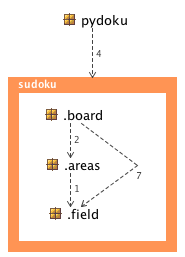
\includegraphics[width=0.3 \textwidth, trim=0 0 0 0, clip=true]{screen_structure}
    \caption{High level dependency between the different modules}
    \label{fig:screen_structure}
\end{figure}

The Structure 101g graph clearly reveals that board uses both areas and fields, where as the area only has relations to the field. The \id{pydoku} modules doesn't do much beside initialise everything. 

\subsection{Dependency Breakdown}

When an arrow is selected Structure 101g shows a overview of the selected dependencies. The figure \vref{fig:screen_dependency_breakdown} shows this for the dependencies between the module \id{pydoku} and the \id{board}. 

\begin{figure}[H]
    \centering
    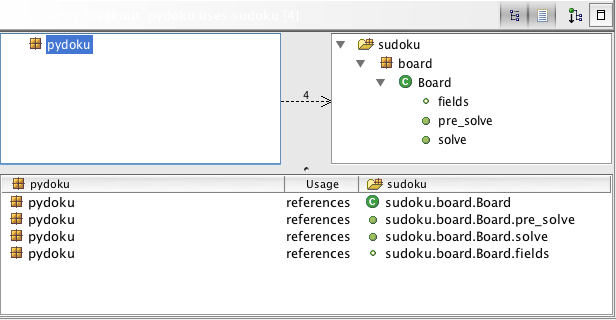
\includegraphics[width=0.7 \textwidth, trim=0 0 0 0, clip=true]{screen_dependency_breakdown}
    \caption{Dependency breakdown}
    \label{fig:screen_dependency_breakdown}
\end{figure}

\subsection{Class Overview}

Structure 101g can also be used to get an overview of the call structure within a single class, as shown in figure \vref{fig:screen_method}. 

\begin{figure}[H]
    \centering
    \fbox{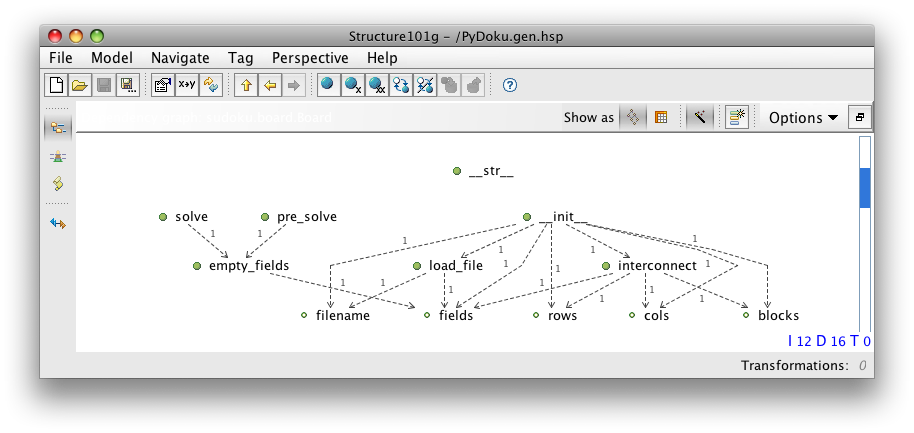
\includegraphics[width=0.98 \textwidth, trim=150 110 120 150, clip=true]{screen_method}}
    \caption{Method call graph within a class}
    \label{fig:screen_method}
\end{figure}

By selecting a single component the analyser further highlights all related components by greying all other components. You see by comparing the  following excerpt of the method \id{load_file} and the figure \vref{fig:screen_method_selected} that the structural analyser was successfully able to identify all dependencies.

\begin{lstlisting}
def load_file(self):
    board_file = file(self.filename)
    i = 0        
    for line in board_file:
        for char in line:
            if char.isspace():
                continue
            value = int(char) if char.isdigit() else None
            self.fields[i].value = value
            i += 1
\end{lstlisting}

\begin{figure}[H]
    \centering
    \fbox{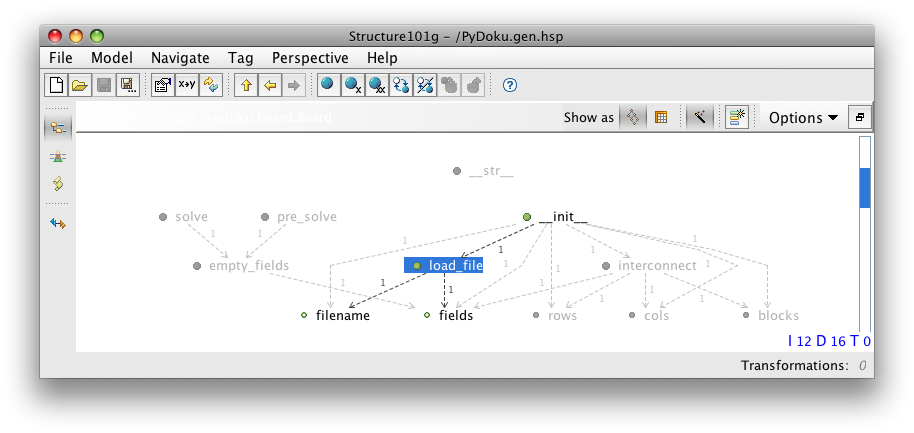
\includegraphics[width=0.98 \textwidth, trim=150 110 120 150, clip=true]{screen_method_selected}}
    \caption{Highlighted method}
    \label{fig:screen_method_selected}
\end{figure}


Structure \\
types (type annotator)\\
Key figures
\todo{maybe describe somewhere that it is very difficult to find all attributes of a given class.}


%%%%%%%%%%%%%%%%%%%%%%%%%%%%%%%%%%%%%%%%%%%%%%%%%%%%%%%%%%%%%%%%%%%%%%%
\chapter{Outlook}

%TODO:  Possible follow-up projects
% Possibilities.. etc.

\section{Type Inference}
\label{outlook_type_inference}

\subsection{Improvements}

The type inference system is in no way perfect and can still be improved in various ways.

The biggest weakness of the goal engine right now is its performance. It could be improved by doing a better caching of goals. For example, the calculation of a function's return type is done for each call even when the called function and the argument types are the same. To avoid this, Ole Agesen's cartesian product algorithm (CPA) could be used \cite{cpa}.

There are other ways to improve the performance. For example when a class uses no attributes, all instances can be treated exactly the same. Or when two instances of a class have the same attribute types, they behave the same way and the analysis could be ``shared''.

Just the elementary built-in types are supported until now. By adding more built-in types and functions, the inferencer would be able to infer more types for more projects. There are also some language features not supported yet, like generator expressions. A similar topic to built-in types is how to handle code which accesses extensions written in C or C++.

Of course there are still bugs and cases where the type inferencer can't infer types. More testing with more real-world projects will reveal these.

% { rstocker: bitte korrigeren und kommentieren
\subsubsection{Code Browser}

A nice idea would be to create a code browser, similar to the type annotator, which would show the source of a project enriched with information available by the type inferencer. Classes, methods and attributes could be linked together so that the user for example could automatically jump to de definition of a method by just clicking on a use of it. Instead of an independent application such functionality could of course also be integrated into a development environment like Eclipse.
% }
\subsection{Possible Uses}

A type inference system can be used for a wide variety of tasks. Some possible use cases which need type inference are for example:

\begin{itemize}
    \item IDE features like code completion, highlighting the occurrences of variable and finding references of classes or methodes
    \item Program exploration tools for browsing source code along with type information
    \item Type checking and compiler optimisations
    \item Increased accuracy for tools which…
    \begin{itemize}
        \item … detect unused/dead code
        \item … look for possible bugs in code (like FindBugs for Java)
    \end{itemize}  
\end{itemize}

Our previous project PEPTIC\cite{peptic2}, where the initial type inference engine originated from, can be ported to the new engine to get the benefits of all the improvements.


%%%%%%%%%%%%%%%%%%%%%%%%%%%%%%%%%%%%%%%%%%%%%%%%%%%%%%%%%%%%%%%%%%%%%%%
\chapter{Quality Assurance}

% \section{Size Over Time}
% \section{Overall Structure}
% \section{Type Inference Engine}
% \section{Quality Assurance Infrastructure}


\section{PyStructure's Structure}

\begin{wrapfigure}{r}{3cm}
    \vspace{-0.7cm}
    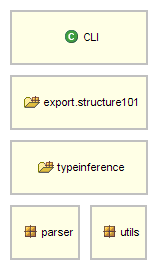
\includegraphics[width=3cm]{architecture/parts}
    \vspace{-1.5cm}
\end{wrapfigure}

PyStructure is designed to be composed of multiple independent parts, as shown on the right. Each of these parts could be in a separate Jar, because a part only depends on parts below it.

From our previous project, PEPTIC, we had to extract the type inference system. We used Structure 101 for this, because it was very useful to see the dependencies of the type inference. With this, the parts could be isolated that we really had to import into our code base.

Keeping the type inferencer as independent as possible from the rest of the project was an important goal for us from the beginning. This independence will be essential when the PEPTIC project will be ported to use the new inferencer.

\section{Infrastructure}

\subsection{Type Inference Tests}

The type inference system was developed in a test-driven manner. To be able to add tests in the easiest way possible, we developed a test framework. Each test case is a Python file in a test directory. Assertions are added by putting markers at the end of lines of interest. An example:

\begin{lstlisting}
def add_one(value):
    value ## type float|int
    return value + 1

add_one ## type function

add_one(41) ## type int
add_one(1.5) ## type float

# Wrong expected type on purpose
add_one(1) ## type float
\end{lstlisting}

The \code{##} is the marker for an assertion, the \texttt{type} is the name of the assertion and the part after that is the expected value.

The implementation is fairly trivial. All the markers in a file are found and a new assertion is created with the type and line number. When the test is run the assertion finds the expression on its line by using an \class{ExpressionAtLineVisitor}. It creates an expression type goal, asks the goal engine to evaluate it and then compares the result with the expected result. If they don't match, a custom error \class{InferencerAssertionError} is thrown with the information about the failure. In the last line of the above example, the expected value was messed up:

\begin{verbatim}
type of <add_one(1)>: expected <float> but was <int> (simple.py:11)
\end{verbatim}

So, adding a new test is a matter of adding a new Python file to the directory, writing some code and adding some assertions by appending \code{## type expected} to a line of an expression. The test will automatically be picked up by the suite and run. This makes it very painless to write tests and that in turn makes it more likely that tests are written.

\subsubsection{Inheritance Tests}

When implementing inheritance support, we needed a way to test the method resolution order (MRO) of classes. So we added a new marker type, \code{mro} which compares the MRO of the expression with the expected value. For example:

\begin{lstlisting}
class A(object): pass
class B(object): pass
class C(object): pass
class X(A): pass
class Y(A): pass
class Z(X,B,Y,C): pass

A ## mro A,object
B ## mro B,object
C ## mro C,object
X ## mro X,A,object
Y ## mro Y,A,object
Z ## mro Z,X,B,Y,A,C,object
\end{lstlisting}

Should the need for other sorts of tests arise, it is just a matter of adding another assertion type.

\subsection{Cobertura}

Cobertura is a test coverage reporting tool. It runs all the tests and collects data about which line of code and which branch was executed and calculates a test coverage metric (e.g. 87~\%). The report is a browsable HTML page where the source code is annotated and coloured to show where more testing is needed.

\subsection{FindBugs}

FindBugs is an automatic fault detection tool that can find problems in Java programs. It uses analysis techniques to identify code patterns known to be problematic – so-called bug patterns. We reviewed all the problems reported by FindBugs and decided to fix them or not. We have fixed all problems which either have been easy or important.

\subsection{Checkstyle}

We used Checkstyle to help us have a uniform Java coding standard. It's a tool which checks if the source code adheres to a certain coding style, for example that opening braces are always on the same line, and issues warnings if it violates it. There's an Eclipse plugin which annotates the source code when there's a violation.

\subsection{Continuous Integration}

All of the above measures to check the code base were automatically run after each commit on our build server. We used CruiseControl for this, which automatically built the whole project, including the documentation. When there was a test failure, e-mails were sent to us that the build had failed, which allowed us to quickly detect and fix problems. It also copied all reports of the above tools to the website, so they could be easily browsed.

As an additionaly gadget, we installed two lava lamps in our workspace, a green one and a red one. On one of our computers, a script was running, which continuously checked the status of the build. If the build failed, the red lava lamp was activated. When everything was okay, the green one was on. This gave us a nice visual feedback about our build status and it was fun.


%%%%%%%%%%%%%%%%%%%%%%%%%%%%%%%%%%%%%%%%%%%%%%%%%%%%%%%%%%%%%%%%%%%%%%%
\chapter{Project Management}

% TODO: PEPTIC

\section{Roadmap}

At the start of the project, we defined four milestones to reach during the development and planned which high-level goals we wanted to reach by then. Detailed goals for the next week were defined at the weekly meetings with our supervisor.

The following was our project plan. Note that the weeks A--E are in fact just two weeks, but because we could work full-time then, we scaled them to correspond to the length of the other weeks.

\begin{figure}[H]
 \centering
 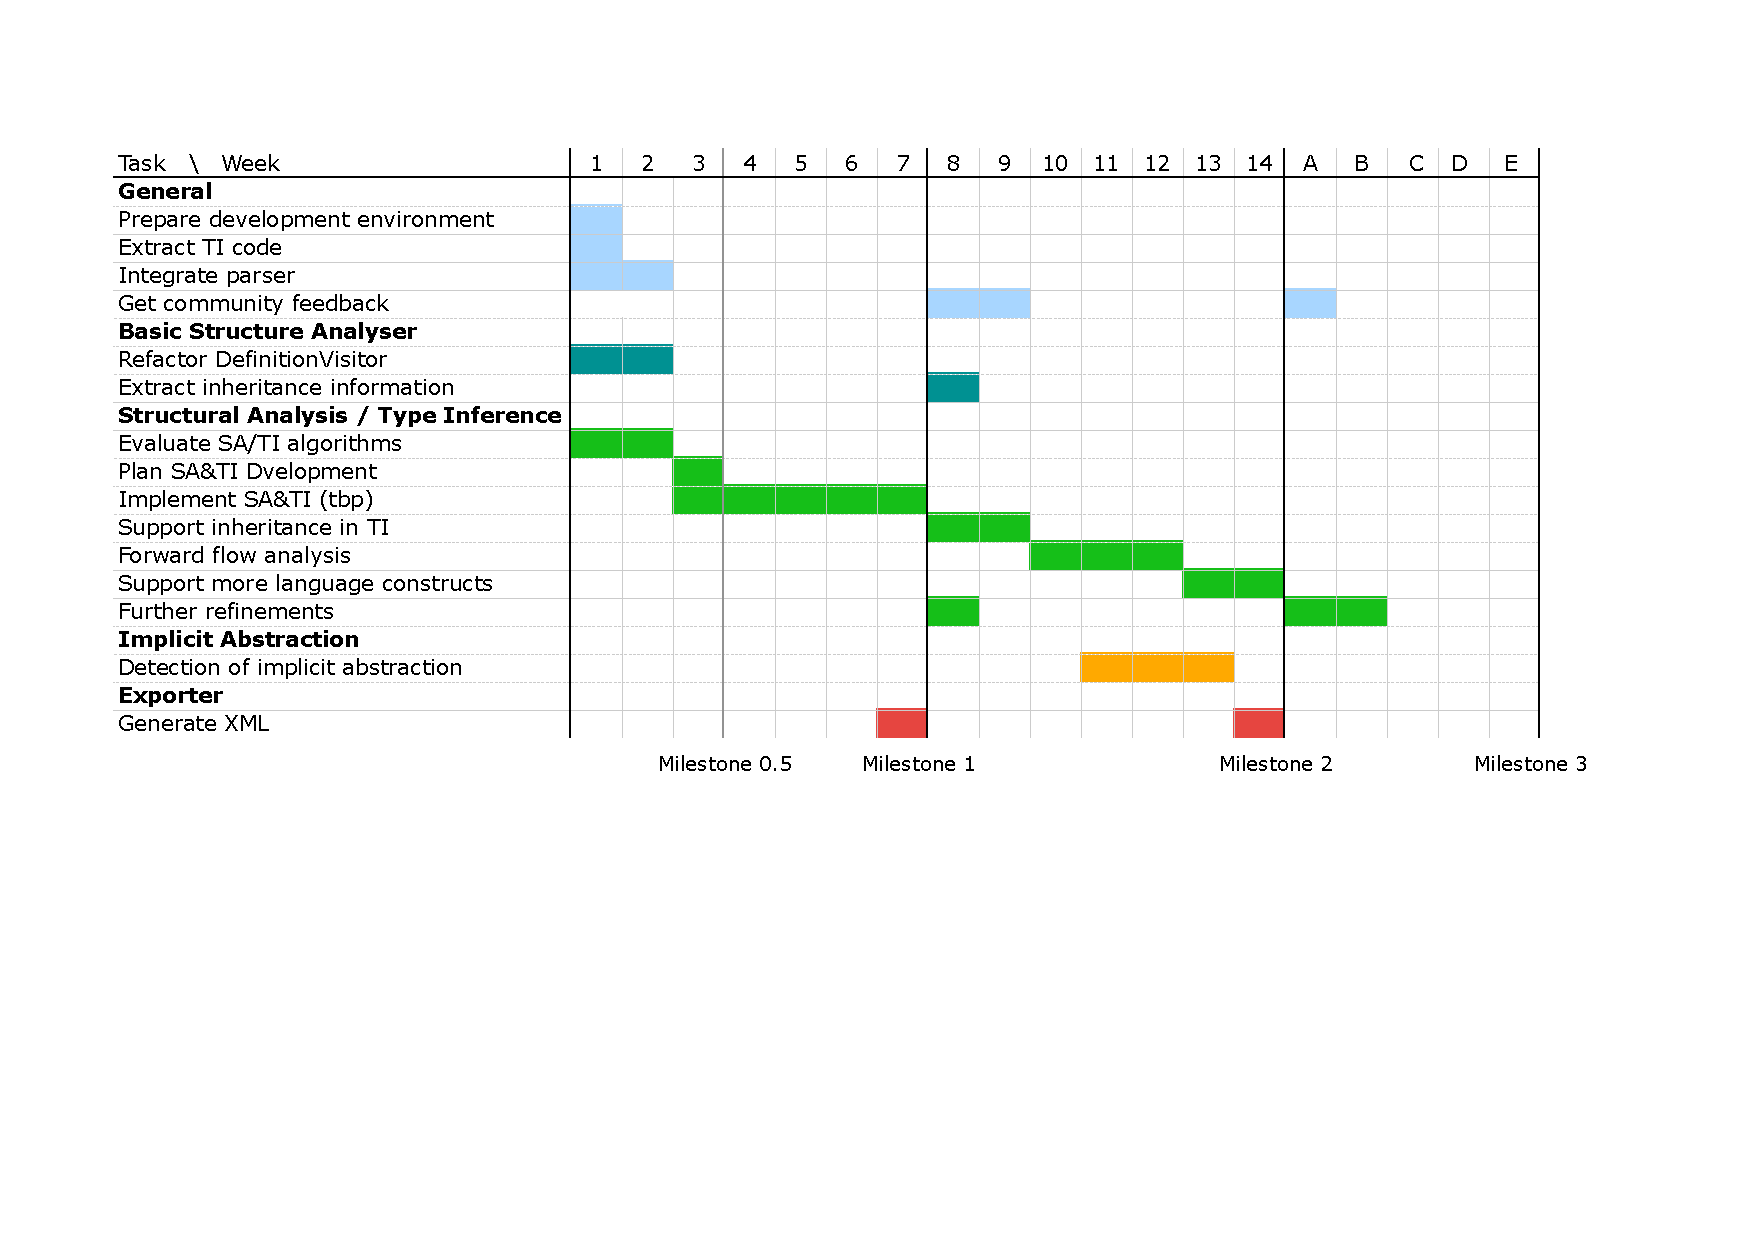
\includegraphics[width=\textwidth, trim=50 220 80 50, clip=true]{project/project-plan-v2}
 \caption{Project plan}
 \label{fig:project_plan}
\end{figure}

In the following, the goals for each milestone are described.

\subsubsection{Milestone 0.5 – Week 3}

\begin{itemize}
    \item Decide whether PEPTIC's goal engine or a new one should be used
\end{itemize}

The goal of the first mini-milestone was deciding whether we should continue using and developing the type inference system from our previous project or whether to base the structural analysis on something new. This meant reading papers and looking for other techniques to do whole-program analysis.

In the end we decided to go with our own goal engine because we wanted to keep it demand-driven and useful for IDEs. Additionally, using another technique would have meant rewriting large parts of the type inference system.

\subsubsection{Milestone 1 – Week 7}

\begin{itemize}
    \item Minimal prototype which understands and analyses basic applications
    \item Important missing features:
    \begin{itemize}
        \item Inheritance
        \item List or other containers
    \end{itemize}
\end{itemize}

This milestone was about producing a prototype that could analyse a basic application and export it to the Structure 101g XML format. Because the prototype relies on all components of PyStructure, the structural analyser and the exporter had to be created and we had to think about how to connect the exporter with the analyser and the analyser with the type inference system.

\subsubsection{Milestone 2 – Week 14}

\begin{itemize}
    \item Second prototype which is able to analyse most common applications
    \item Support for lists and inheritance
\end{itemize}

This milestone was primarily focused on two hard type inference features, inheritance and the analysis of container element types (see \vref{container_element_types}).

% TODO: mehr schreiben

\subsubsection{Milestone 3 – Week 16}

\begin{itemize}
    \item Final version which is usable for real-world projects
\end{itemize}

For the final milestone, the goal was to add support for built-in types and other refinements to make the system usable for real-world projects.

% TODO: mehr schreiben

 (Problems, important decisions) \\
 Our Experiences

\section{Used Licence}

We decided to use the LGPL (version 2 or later) for the PyStructure project for the following reasons:

\begin{itemize}
    \item It is a Free Software licence and GPL-compatible.
    \item Proprietary applications can still use the library.
    \item Modifications to the library itself have to be released under the LGPL.
\end{itemize}

\section{Parts of Documentation from Previous Project}

Some parts of this document were taken from our previous project:

\begin{itemize}
    \item 70~\% of section \vref{connecting_definitions_and_uses}, \emph{Connecting Definitions and Uses}
\end{itemize}

\section{Working Hours}

The diagram below shows the hours per week we worked on this bachelor thesis. The orange line shows the recommended number of hours and the bars are our actual hours. The first 14 weeks were in the semester alongside the lectures and 20 hours of work per week were recommended. The last 2 weeks we could work full time, which means 45 hours each week.

\begin{figure}[H]
 \centering
 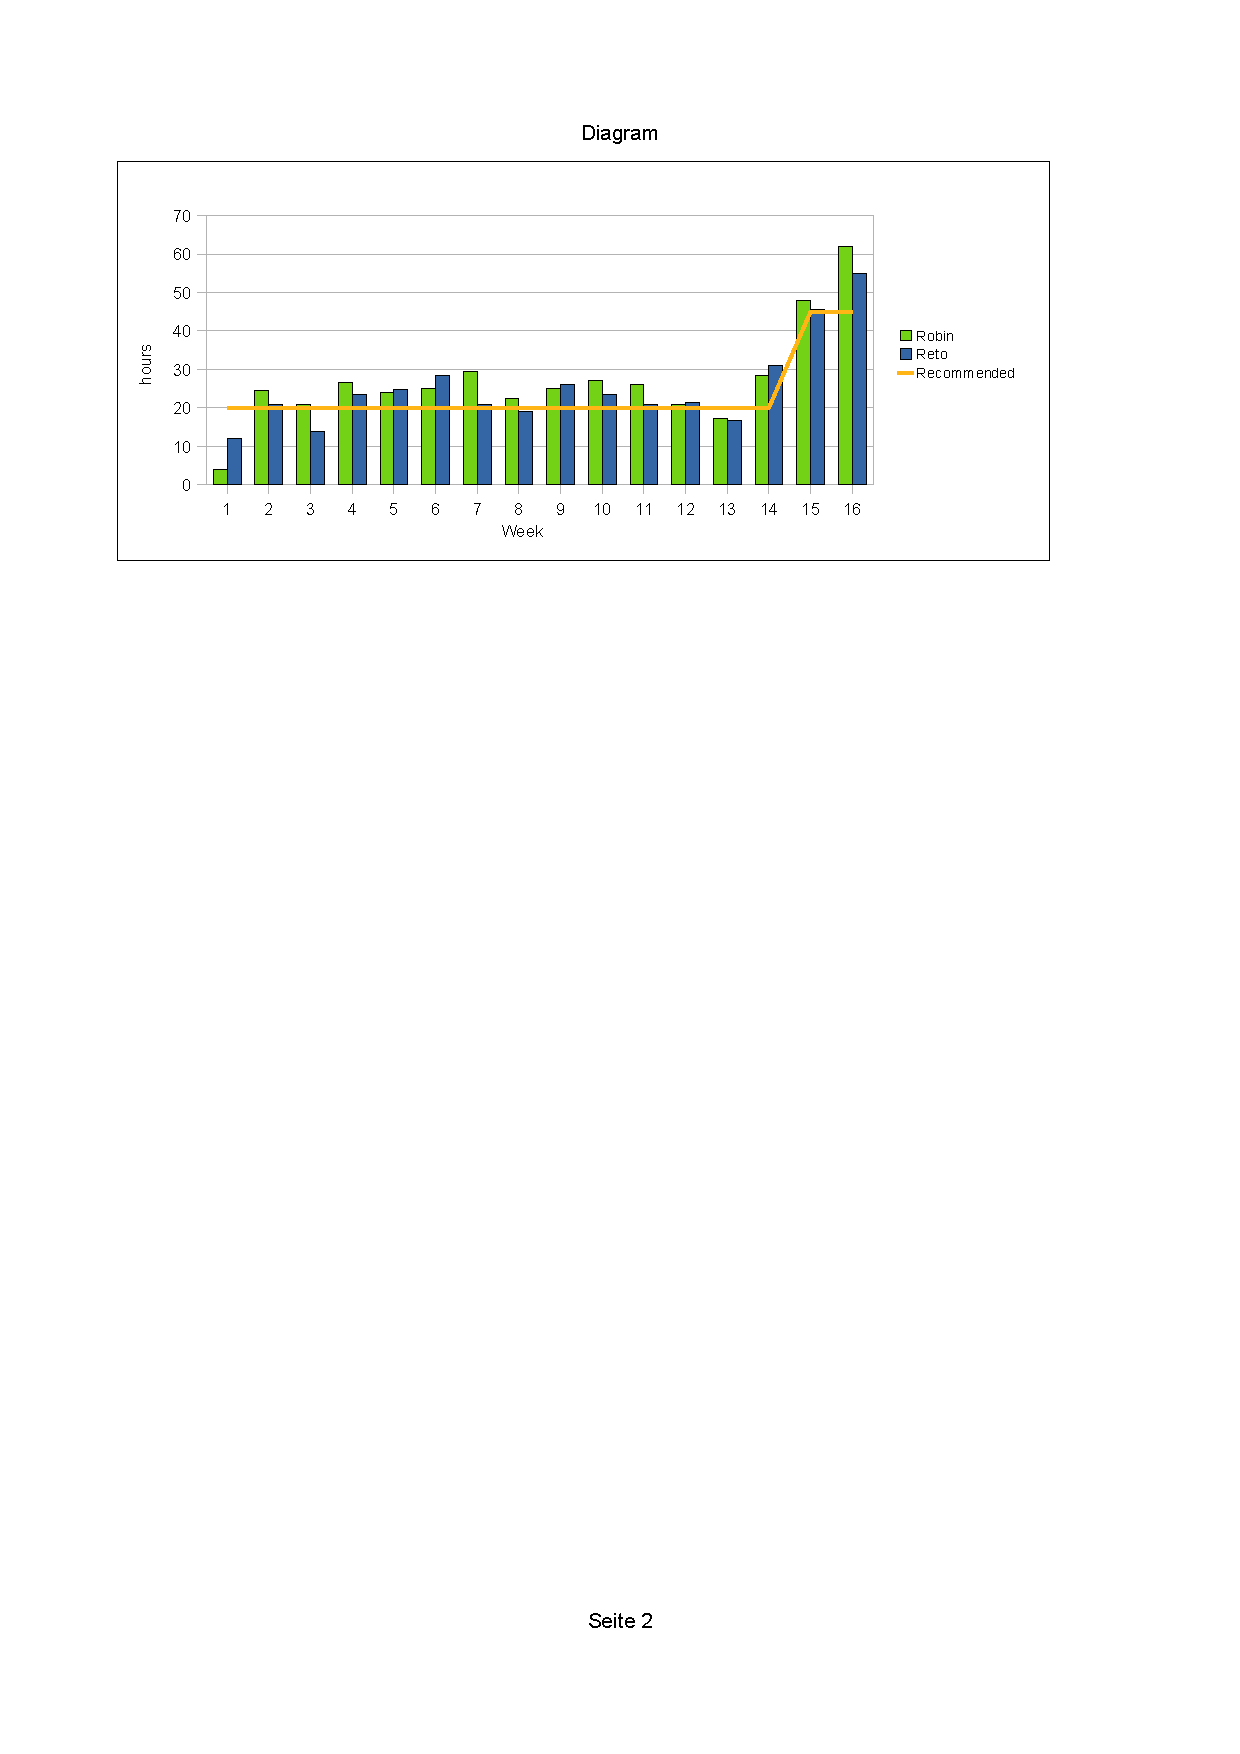
\includegraphics[width=\textwidth, trim=50 570 90 70, clip=true]{project/working_hours}
 \caption{Diagram of working hours per week}
 \label{fig:working_hours}
\end{figure}

\section{Thanks}

\begin{itemize}
    \item to Peter Sommerlad and Thomas Corbat for their support during the project
    \item to Christian Bachmann for the life-saving coffee machine in our study room. 
\end{itemize}


%%%%%%%%%%%%%%%%%%%%%%%%%%%%%%%%%%%%%%%%%%%%%%%%%%%%%%%%%%%%%%%%%%%%%%%

%%%%%%%%%%%%%%%%%%%%%%%%%%%%%%%%%%%%%%%%%%%%%%%%%%%%%%%%%%%%%%%%%%%%%%%
\setcounter{secnumdepth}{-1}
\chapter{Appendix}
\pagenumbering{Alph}

\section{Evaluators}


\begin{itemize}
    \item References
    \begin{itemize}
        \item Attribute References
        \item Calculate Type Hierarchy
        \item Class References
        \item Function References
        \item Method References
        \item Possible Attribute References
        \item Possible References
        \item Variable Reference
    \end{itemize}
    \item Types
    \begin{itemize}
        \item Argument Type
        \item Assign Type
        \item Attribute Type
        \item Bin Op Type
        \item Bool Op Type
        \item Builtin Type
        \item Call Type
        \item Class Attribute Type
        \item Definition Type
        \item Dict Type
        \item Display Type
        \item If Exp Type
        \item Implicit Import Type
        \item Import Type
        \item List Comp Type
        \item List Type
        \item Loop Variable Type
        \item Return Type
        \item Simple Expression Type
        \item Subscript Type
    \end{itemize}
    \item Misc
    \begin{itemize}
        \item Fixed Result
        \item Method Resolution Order
        \item Method Resolve
    \end{itemize}
\end{itemize}

\listoffigures

\bibliographystyle{alphadin}
\bibliography{bibliography}


\end{document}
